% Gerado automaticamente por atualizar_apresentacao.py — NÃO editar à mão.
\documentclass[aspectratio=169,11pt]{beamer}

% ------------------------------------------------
% TEMA MINIMALISTA AMARELO — modo escuro (Variação 4B)
% ------------------------------------------------
\usepackage{xcolor}
\usepackage{colortbl}

\definecolor{myyellow}{RGB}{255,200,40}
\definecolor{grafite}{RGB}{26,26,26}
\definecolor{textoclaro}{RGB}{230,230,230}

\setbeamercolor{background canvas}{bg=grafite}
\setbeamercolor{normal text}{fg=textoclaro}
\setbeamercolor{title}{fg=myyellow}
\setbeamercolor{frametitle}{fg=myyellow}
\setbeamercolor{structure}{fg=myyellow}

\setbeamertemplate{navigation symbols}{}

% Linhas da tabela (booktabs) claras, visíveis no fundo grafite
\arrayrulecolor{textoclaro}

% ------------------------------------------------
% PACOTES
% ------------------------------------------------
\usepackage[utf8]{inputenc}
\usepackage[T1]{fontenc}
\usepackage{lmodern}
\usepackage[brazil]{babel}
\usepackage{graphicx}
\usepackage{booktabs}
\usepackage{adjustbox}

% ------------------------------------------------
% INFO
% ------------------------------------------------
\title{Classificação Automática de Modulações}
\subtitle{Aplicações em Internet das Coisas}
\author{João Marco Pereira}
\institute{CEFET/RJ}
\date{Resultados parciais por grupo de modulação --- 4 de agosto de 2026}

\begin{document}

\begin{frame}
  \titlepage
\end{frame}

\begin{frame}{Contexto e motivação}
  \begin{itemize}\setlength{\itemsep}{2mm}
    \item \textbf{Internet das Coisas (IoT):} dispositivos heterogêneos compartilham o espectro de RF usando diferentes esquemas de modulação.
    \item \textbf{Reconhecimento automático de modulação (AMR):} identificar a modulação do sinal recebido --- base para monitoramento espectral, comunicações cognitivas, segurança e gerenciamento de redes.
    \item Abordagens clássicas dependem de extração manual de características e de pressupostos sobre o canal, limitando a generalização.
    \item \textbf{Aprendizado profundo:} extração de características e classificação aprendidas de forma conjunta (fim-a-fim), diretamente das amostras I/Q.
  \end{itemize}
\end{frame}

\begin{frame}{Objetivos}
  \textbf{Objetivo geral:} desenvolver e avaliar modelos de aprendizado de máquina para classificar automaticamente o tipo de modulação de um sinal recebido em ambiente IoT.
  \vspace{3mm}

  \textbf{Objetivos específicos:}
  \begin{itemize}\setlength{\itemsep}{2mm}
    \item estudar técnicas de aprendizado de máquina aplicadas à classificação de sinais de comunicação;
    \item implementar e treinar modelos de aprendizado supervisionado para identificação de modulações;
    \item avaliar o desempenho dos modelos em cenários com ruído e diferentes condições de canal.
  \end{itemize}
\end{frame}

\begin{frame}{Bases de dados consideradas}
  \begin{itemize}\setlength{\itemsep}{3mm}
    \item \textbf{RadioModRec-1:} 15 modulações digitais; canais AWGN, Rayleigh e Rician; SNR de $-20$ a $+20$~dB.
    \item \textbf{AugMod (Pythagore-Mod-Reco):} amostras I/Q em HDF5; 7 classes de modulação e 5 níveis de SNR.
    \item \textbf{DeepSig RadioML 2018.01A} (\emph{selecionada}): $\approx$2,5 milhões de exemplos; 24 modulações analógicas e digitais; séries de 1024 amostras I/Q; SNR de $-20$ a $+30$~dB com efeitos realistas de canal.
  \end{itemize}
\end{frame}

\begin{frame}{Etapas anteriores --- modelos avaliados}
  Treinamento inicial com amostras de SNR 20 e 30~dB (24 classes):
  \vspace{2mm}
  \begin{itemize}\setlength{\itemsep}{2mm}
    \item \textbf{MLP} (vetores 1D das amostras I/Q; \emph{Grid Search}): acurácia $\approx$29\%.
    \item \textbf{LightGBM} (\emph{gradient boosting}; \emph{Randomized Search}): acurácia $\approx$44\%.
    \item \textbf{CNN 1D básica} (séries temporais I/Q): acurácia $\approx$78,6\%.
  \end{itemize}
  \vspace{3mm}
  A CNN motivou a etapa seguinte: análise por grupos de modulação e busca de arquiteturas.
\end{frame}

\begin{frame}{Arquitetura da CNN de referência}
  \centering
  \scriptsize
  \begin{adjustbox}{max width=\textwidth, max totalheight=0.8\textheight}
  \begin{tabular}{lcr}
    \toprule
    \textbf{Camada (tipo)} & \textbf{Dimensão de saída} & \textbf{Parâmetros} \\
    \midrule
    Conv1D (64 filtros)   & (None, 1022, 64) & 448 \\
    MaxPooling1D          & (None, 511, 64)  & 0 \\
    Dropout               & (None, 511, 64)  & 0 \\
    Conv1D (128 filtros)  & (None, 509, 128) & 24.704 \\
    MaxPooling1D          & (None, 254, 128) & 0 \\
    Dropout               & (None, 254, 128) & 0 \\
    Conv1D (256 filtros)  & (None, 252, 256) & 98.560 \\
    MaxPooling1D          & (None, 126, 256) & 0 \\
    Dropout               & (None, 126, 256) & 0 \\
    Flatten               & (None, 32.256)   & 0 \\
    Dense (512 neurônios) & (None, 512)      & 16.515.584 \\
    Dropout               & (None, 512)      & 0 \\
    Dense (24 classes)    & (None, 24)       & 12.312 \\
    \midrule
    \multicolumn{2}{r}{\textbf{Total de parâmetros treináveis}} & \textbf{16.651.608} \\
    \bottomrule
  \end{tabular}
  \end{adjustbox}
\end{frame}
\begin{frame}{Comparação entre modelos (etapas anteriores)}
  \centering
  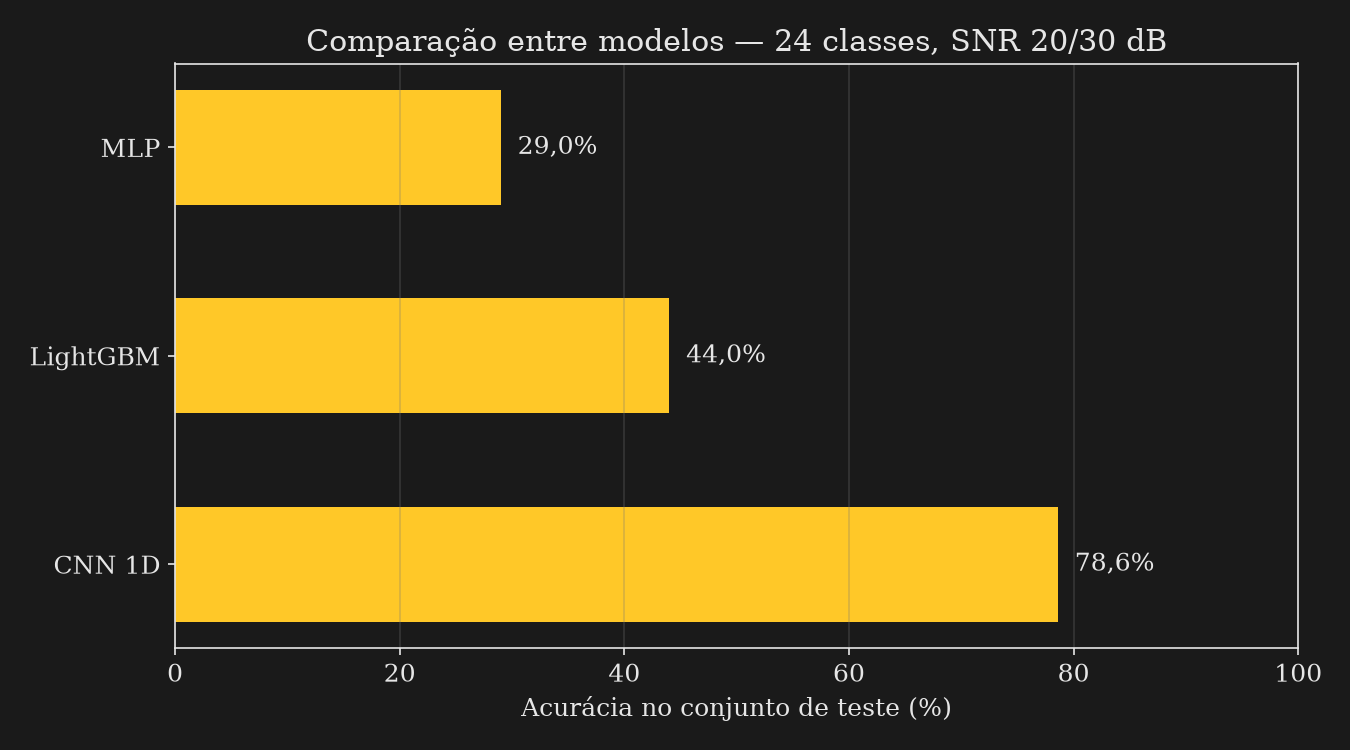
\includegraphics[width=0.96\textwidth,height=0.82\textheight,keepaspectratio]{kfold_analysis/comparacao_modelos.png}
\end{frame}

\begin{frame}{Grupos de modulação (RadioML 2018.01A)}
  \centering
  \begin{tabular}{ll}
    \toprule
    \textbf{Grupo} & \textbf{Modulações} \\
    \midrule
    ASK  & OOK, 4ASK, 8ASK \\
    PSK  & BPSK, QPSK, 8PSK, 16PSK, 32PSK, GMSK, OQPSK \\
    APSK & 16APSK, 32APSK, 64APSK, 128APSK \\
    QAM  & 16QAM, 32QAM, 64QAM, 128QAM, 256QAM \\
    AM   & AM-SSB-WC, AM-SSB-SC, AM-DSB-WC, AM-DSB-SC \\
    FM   & FM \\
    \bottomrule
  \end{tabular}
  \vspace{3mm}

  Filtragem por SNR (0 a $+30$~dB); divisão 60/20/20 (treino/validação/teste) estratificada; \emph{seed} fixa (42).
\end{frame}
\begin{frame}{Modelo combinado (2 estágios) --- acurácia $\times$ SNR (24 classes)}
  \centering
  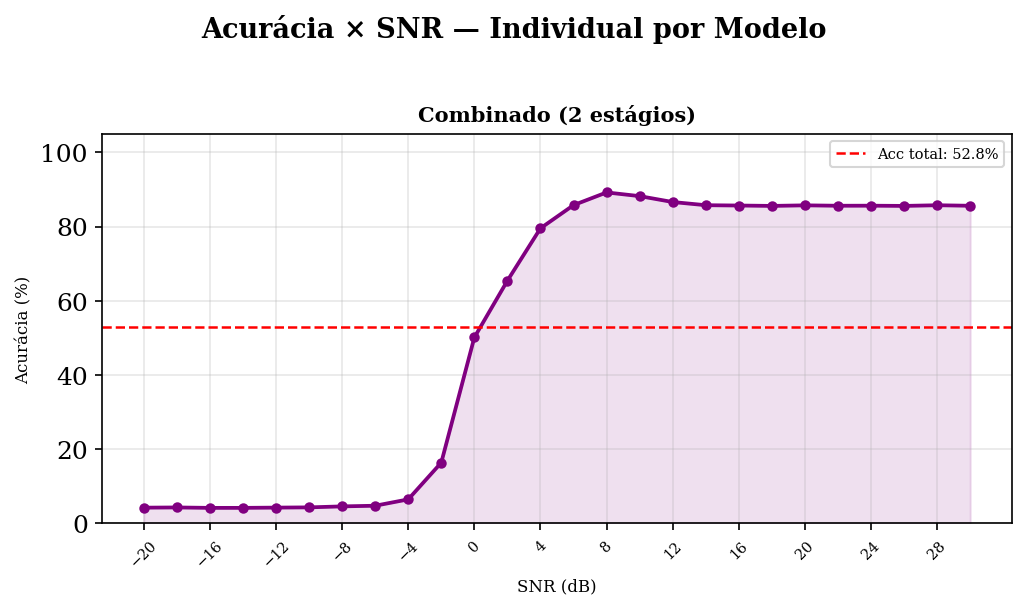
\includegraphics[width=0.96\textwidth,height=0.82\textheight,keepaspectratio]{report_figs/accuracy_vs_snr_individual.png}
\end{frame}
\begin{frame}{Modelo combinado (2 estágios) --- matriz de confusão (24 classes)}
  \centering
  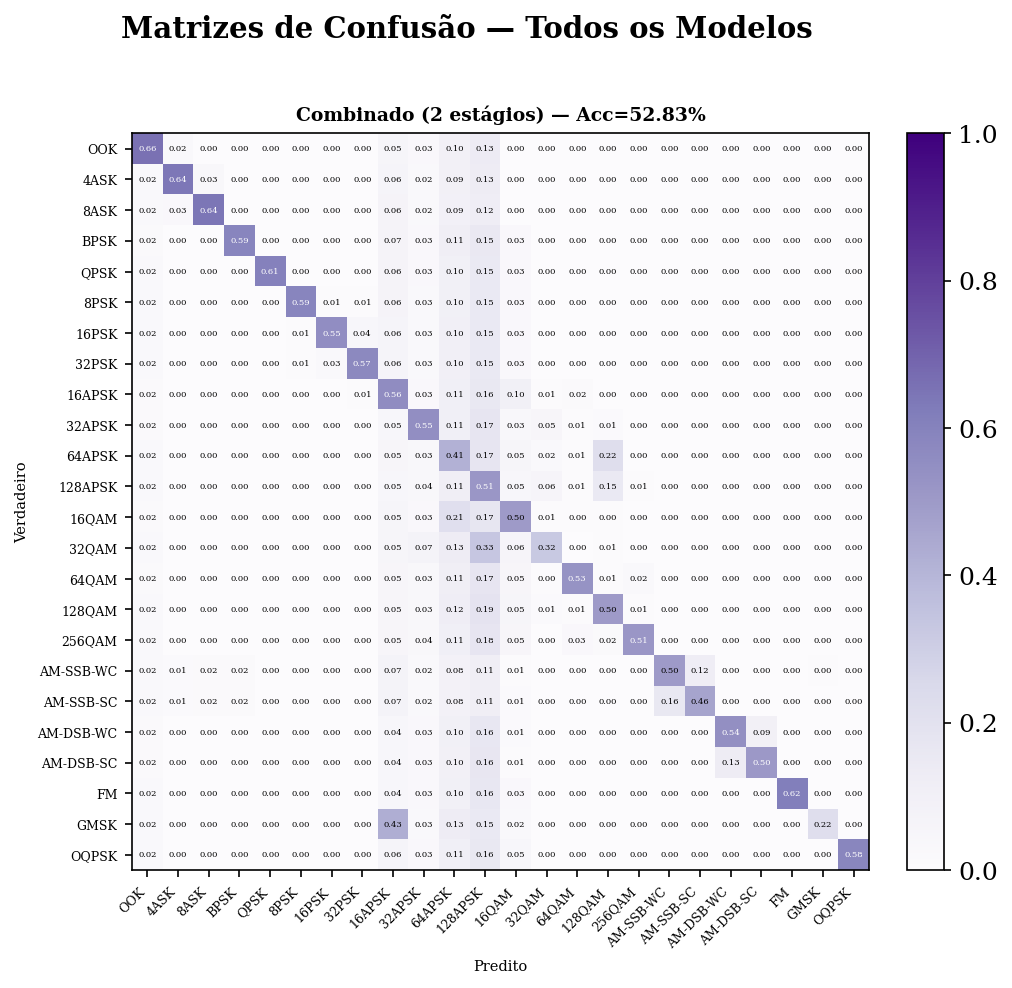
\includegraphics[width=0.96\textwidth,height=0.82\textheight,keepaspectratio]{report_figs/confusion_matrices_all.png}
\end{frame}
\begin{frame}{Modelo de 2 estágios --- avaliação do grupo ASK}
  \centering
  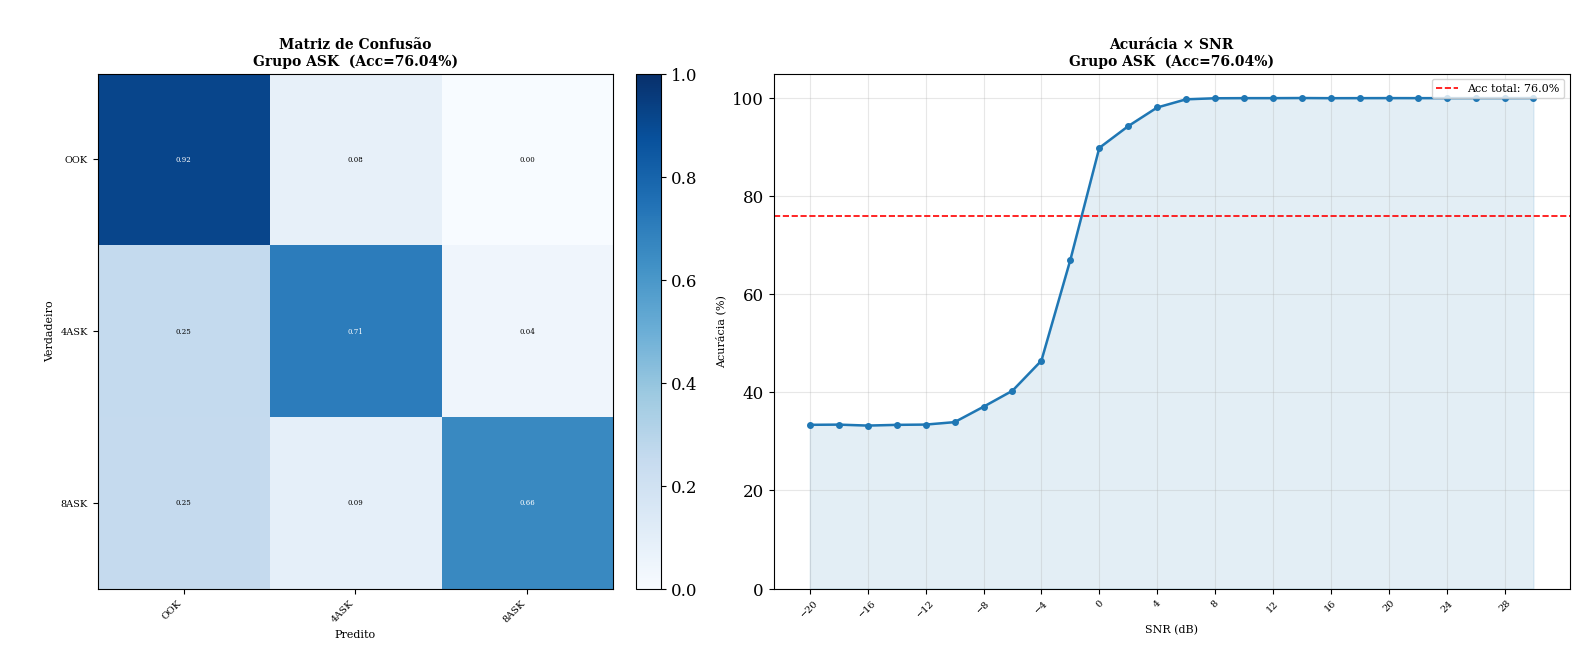
\includegraphics[width=0.96\textwidth,height=0.82\textheight,keepaspectratio]{report_figs/avaliacao_2estagios_ASK.png}
\end{frame}
\begin{frame}{Modelo de 2 estágios --- avaliação do grupo PSK}
  \centering
  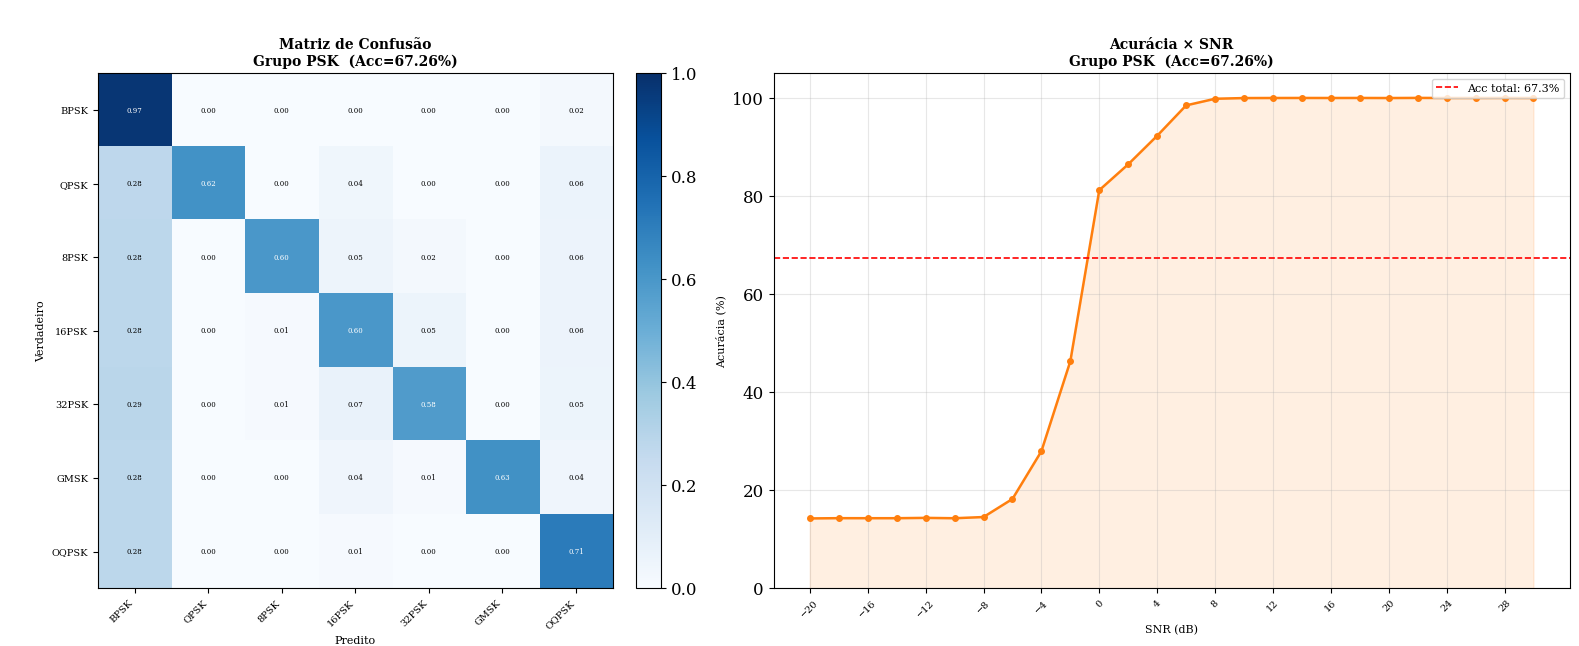
\includegraphics[width=0.96\textwidth,height=0.82\textheight,keepaspectratio]{report_figs/avaliacao_2estagios_PSK.png}
\end{frame}
\begin{frame}{Modelo de 2 estágios --- avaliação do grupo APSK}
  \centering
  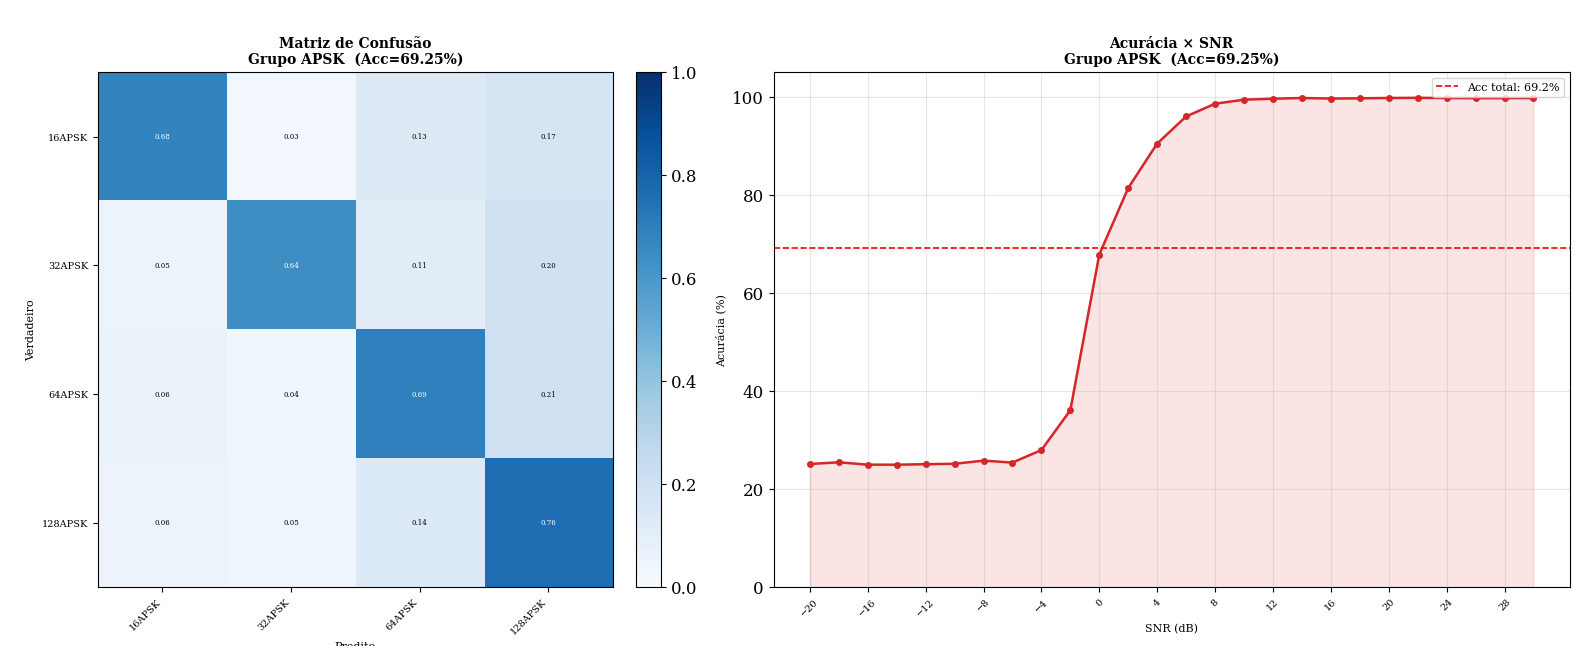
\includegraphics[width=0.96\textwidth,height=0.82\textheight,keepaspectratio]{report_figs/avaliacao_2estagios_APSK.png}
\end{frame}
\begin{frame}{Modelo de 2 estágios --- avaliação do grupo QAM}
  \centering
  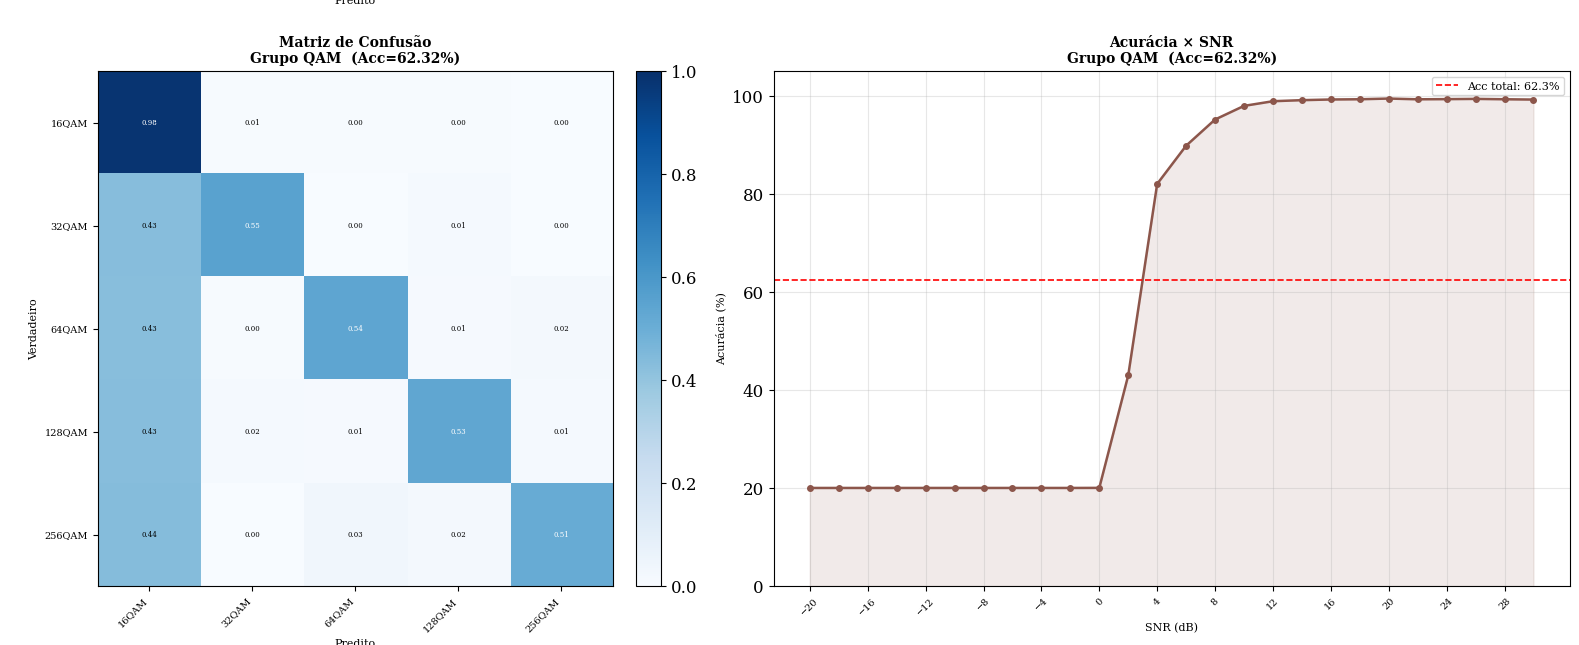
\includegraphics[width=0.96\textwidth,height=0.82\textheight,keepaspectratio]{report_figs/avaliacao_2estagios_QAM.png}
\end{frame}
\begin{frame}{Modelo de 2 estágios --- avaliação do grupo AM}
  \centering
  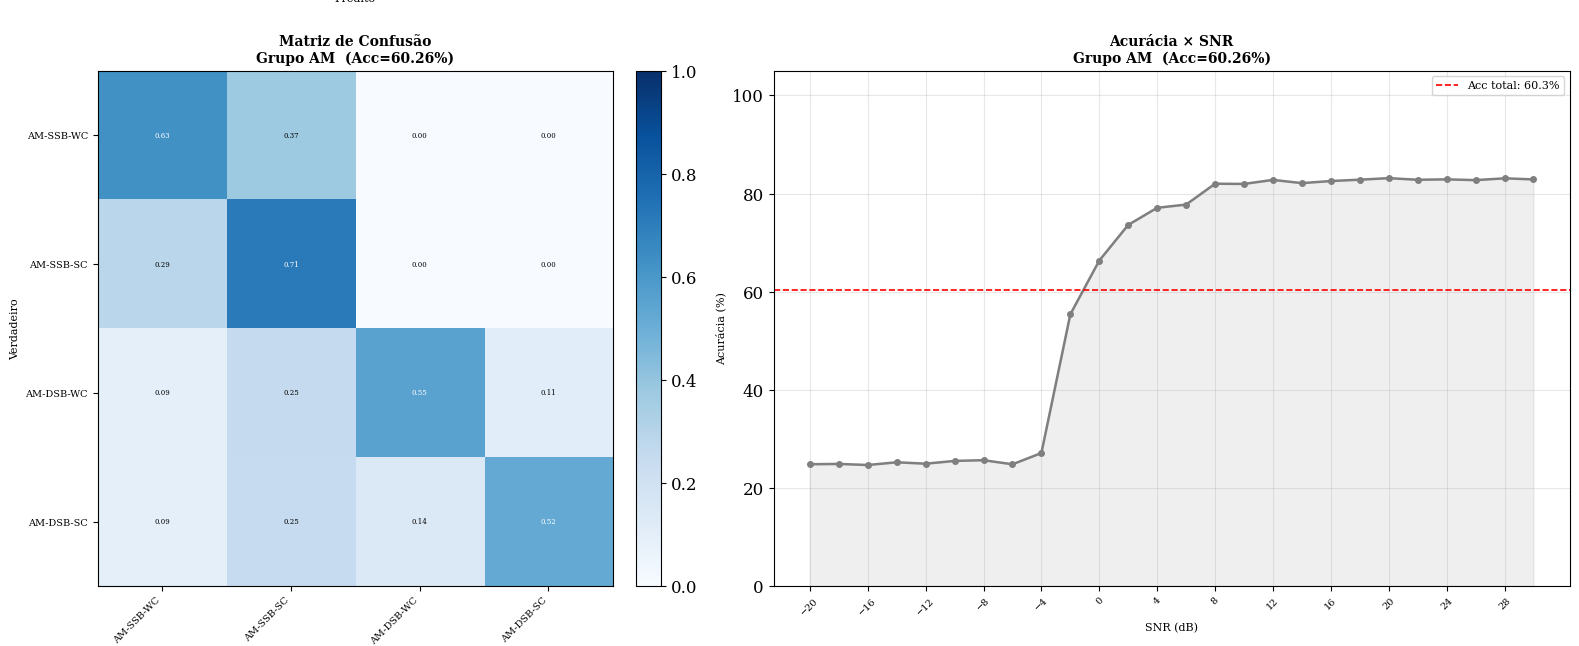
\includegraphics[width=0.96\textwidth,height=0.82\textheight,keepaspectratio]{report_figs/avaliacao_2estagios_AM.png}
\end{frame}
\begin{frame}{Modelo de 2 estágios --- avaliação geral (6 grupos)}
  \centering
  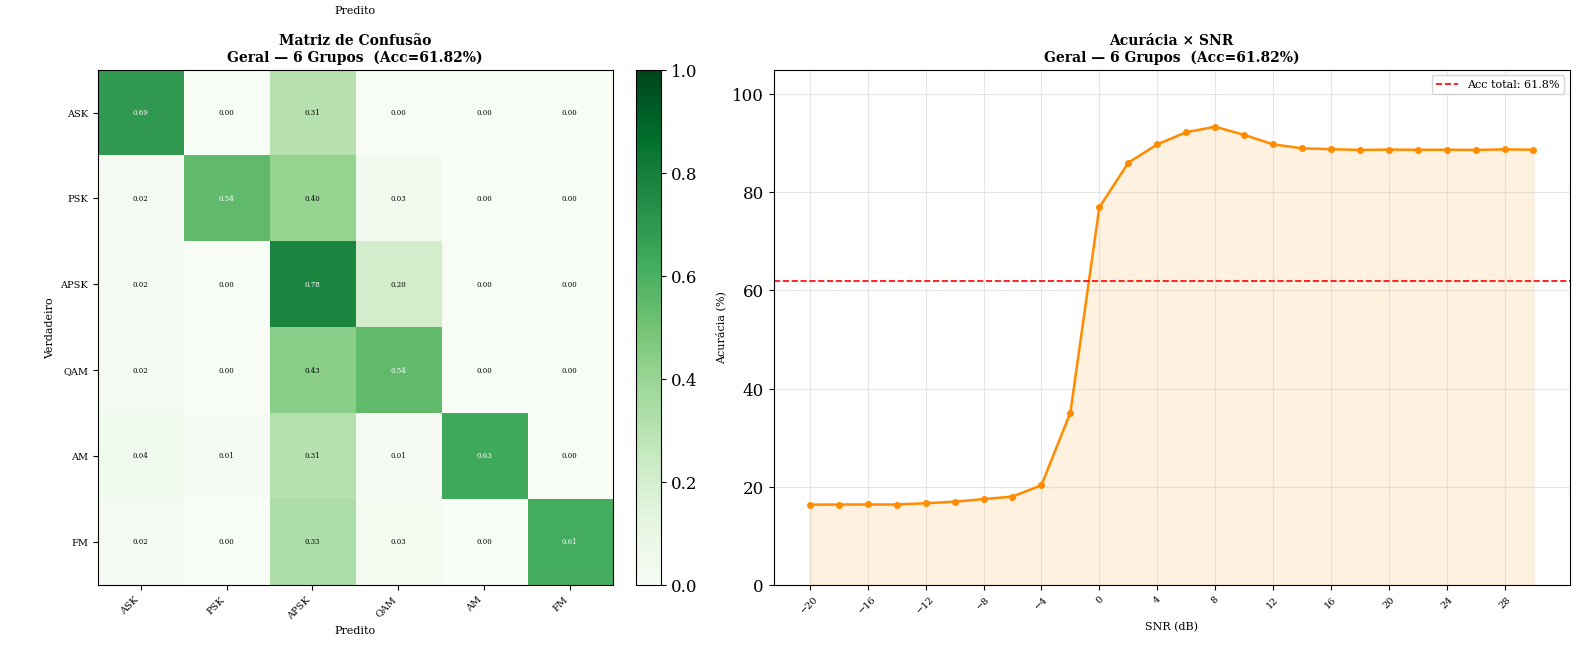
\includegraphics[width=0.96\textwidth,height=0.82\textheight,keepaspectratio]{report_figs/avaliacao_2estagios_GERAL.png}
\end{frame}

\begin{frame}{Metodologia}
  \begin{itemize}\setlength{\itemsep}{2mm}
    \item \textbf{Dataset:} RadioML 2018.01A (sinais I/Q de 1024 amostras, 24 modulações, vários SNRs).
    \item \textbf{Modelo base:} CNN 1D (blocos Conv1d + BatchNorm + ReLU + MaxPool) seguida de classificador denso.
    \item \textbf{Busca de arquitetura:} variação do número de camadas convolucionais e de filtros por camada (ex.: \texttt{2L\_32-64} = 2 camadas com 32 e 64 filtros).
    \item \textbf{Validação:} k-fold com 5 folds por arquitetura; métrica = melhor acurácia de validação de cada fold.
    \item Treino com \emph{early stopping} baseado na paciência do \emph{scheduler} (ReduceLROnPlateau).
    \item Resultados sincronizados via Google Drive e analisados em modo somente leitura.
  \end{itemize}
\end{frame}

\begin{frame}{Status geral da busca}
  \centering
  \small
  \begin{adjustbox}{max width=\textwidth}
  \begin{tabular}{lrrlrr}
    \toprule
    \textbf{Grupo} & \textbf{Arqs.} & \textbf{Folds} & \textbf{Melhor arquitetura} & \textbf{Média (\%)} & \textbf{Máx (\%)} \\
    \midrule
    ASK* & 12 & 60 & \texttt{6L\_64-64-128-128-256-512\_mixpool} & 97,80 & 97,93 \\
    PSK* & 12 & 60 & \texttt{2L\_32-64} & 68,21 & 83,51 \\
    APSK & 5 & 24 & \texttt{2L\_32-64} & 25,00 & 25,01 \\
    QAM & 1 & 5 & \texttt{2L\_32-64} & 20,00 & 20,00 \\
    AM & 12 & 60 & \texttt{2L\_64-128} & 77,99 & 79,40 \\
    FM & --- & --- & \multicolumn{3}{l}{sem resultados até o momento} \\
    \bottomrule
  \end{tabular}
  \end{adjustbox}
  \par\vspace{2mm}{\scriptsize * dados do relatório (backups locais); não disponíveis no Drive.}
\end{frame}
\begin{frame}{ASK --- acurácia por época (melhor fold de cada arquitetura) (figura do relatório)}
  \centering
  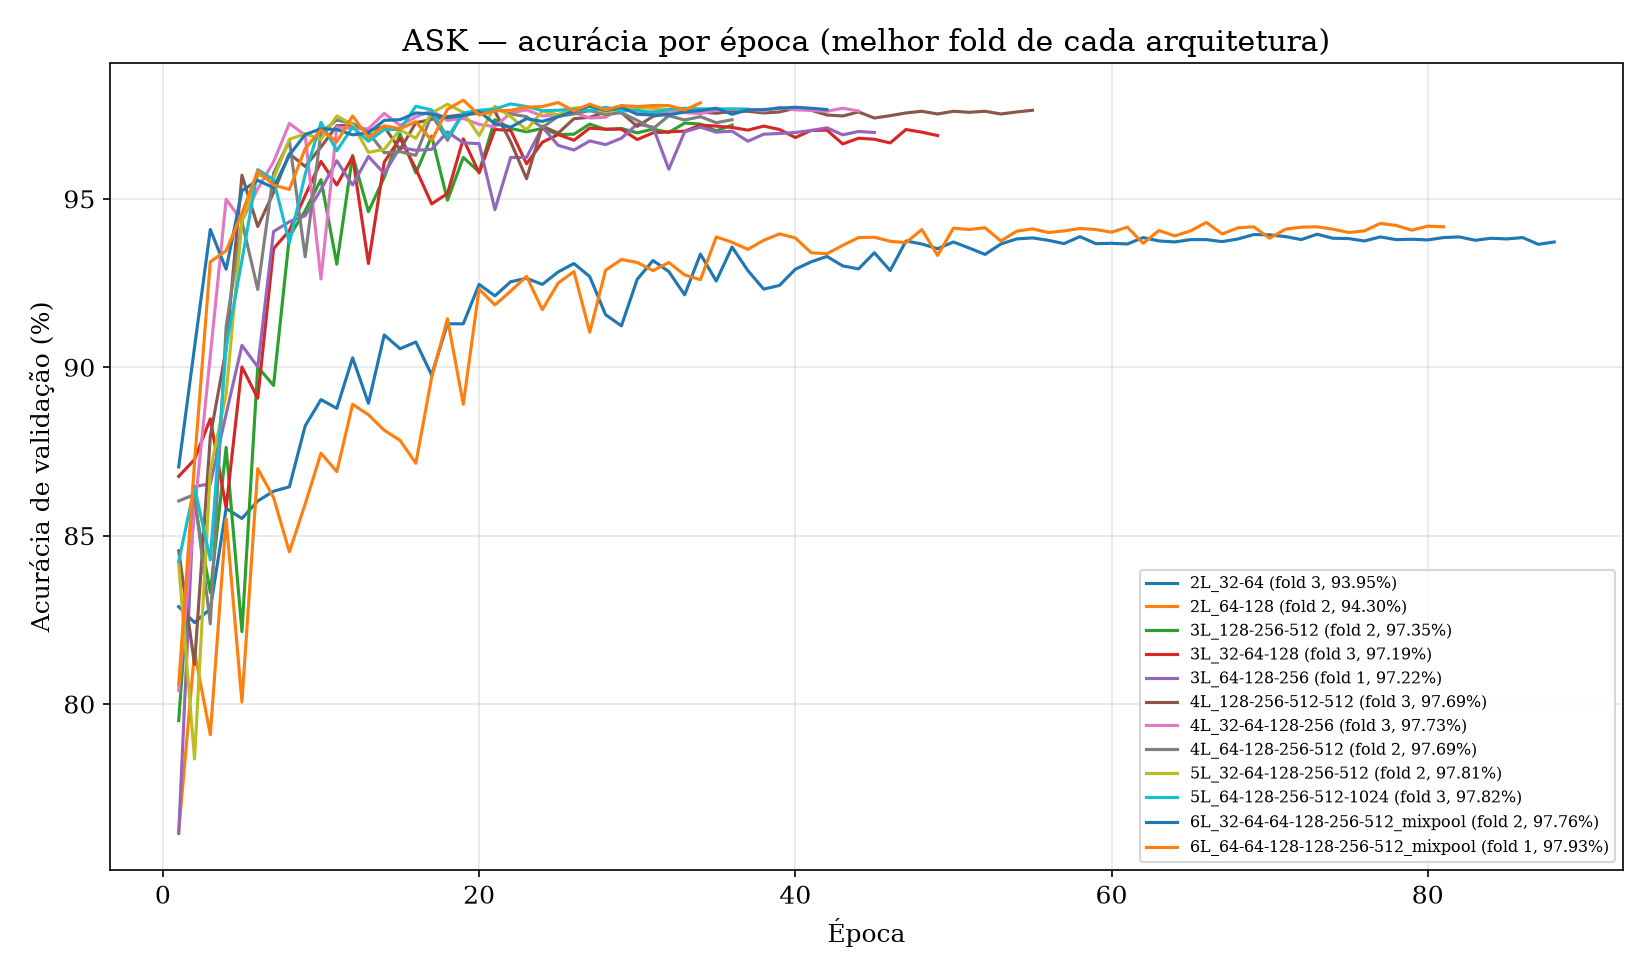
\includegraphics[width=0.96\textwidth,height=0.82\textheight,keepaspectratio]{report_figs/ASK_epochs_best_fold_light.png}
\end{frame}
\begin{frame}{ASK --- número de parâmetros $\times$ acurácia média (figura do relatório)}
  \centering
  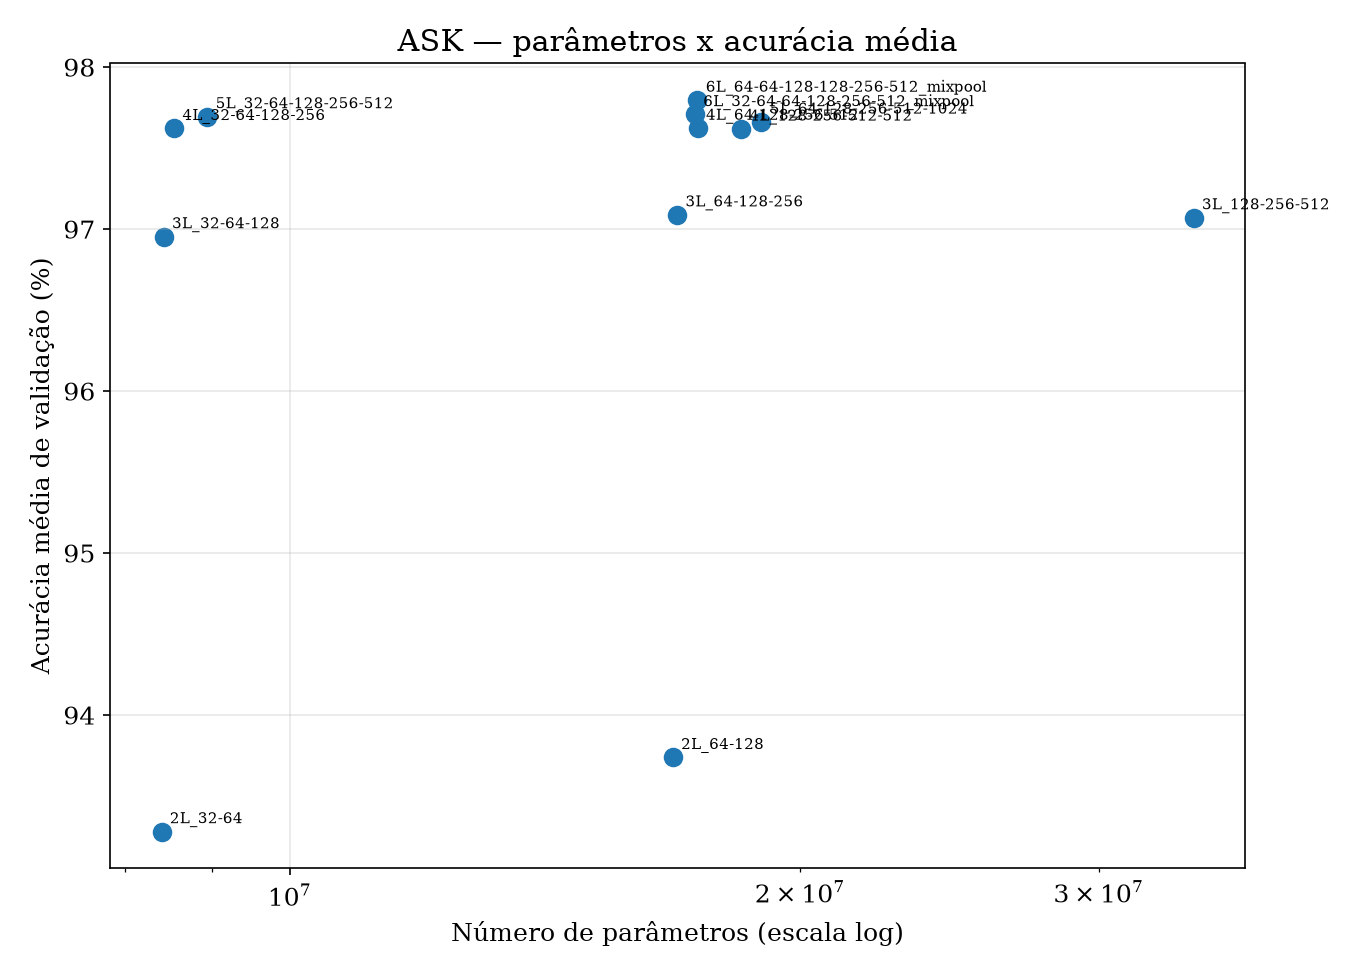
\includegraphics[width=0.96\textwidth,height=0.82\textheight,keepaspectratio]{report_figs/ASK_params_vs_acc_light.png}
\end{frame}
\begin{frame}{PSK --- acurácia por época (melhor fold de cada arquitetura) (figura do relatório)}
  \centering
  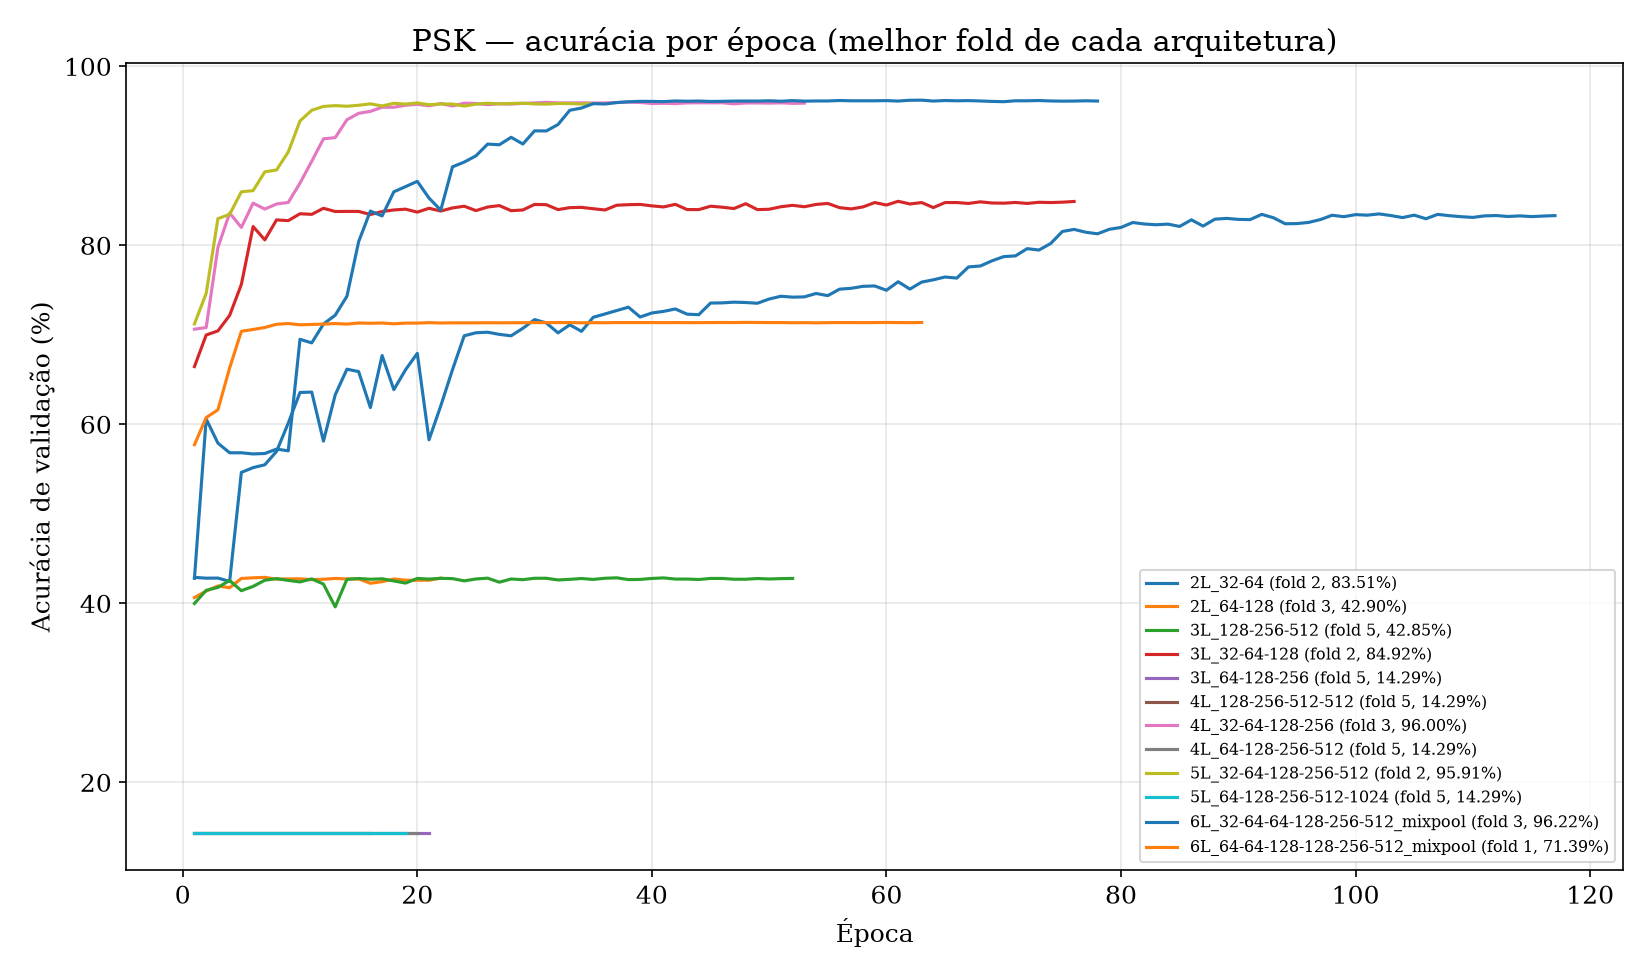
\includegraphics[width=0.96\textwidth,height=0.82\textheight,keepaspectratio]{report_figs/PSK_epochs_best_fold_light.png}
\end{frame}
\begin{frame}{PSK --- acurácia por época (pior fold de cada arquitetura) (figura do relatório)}
  \centering
  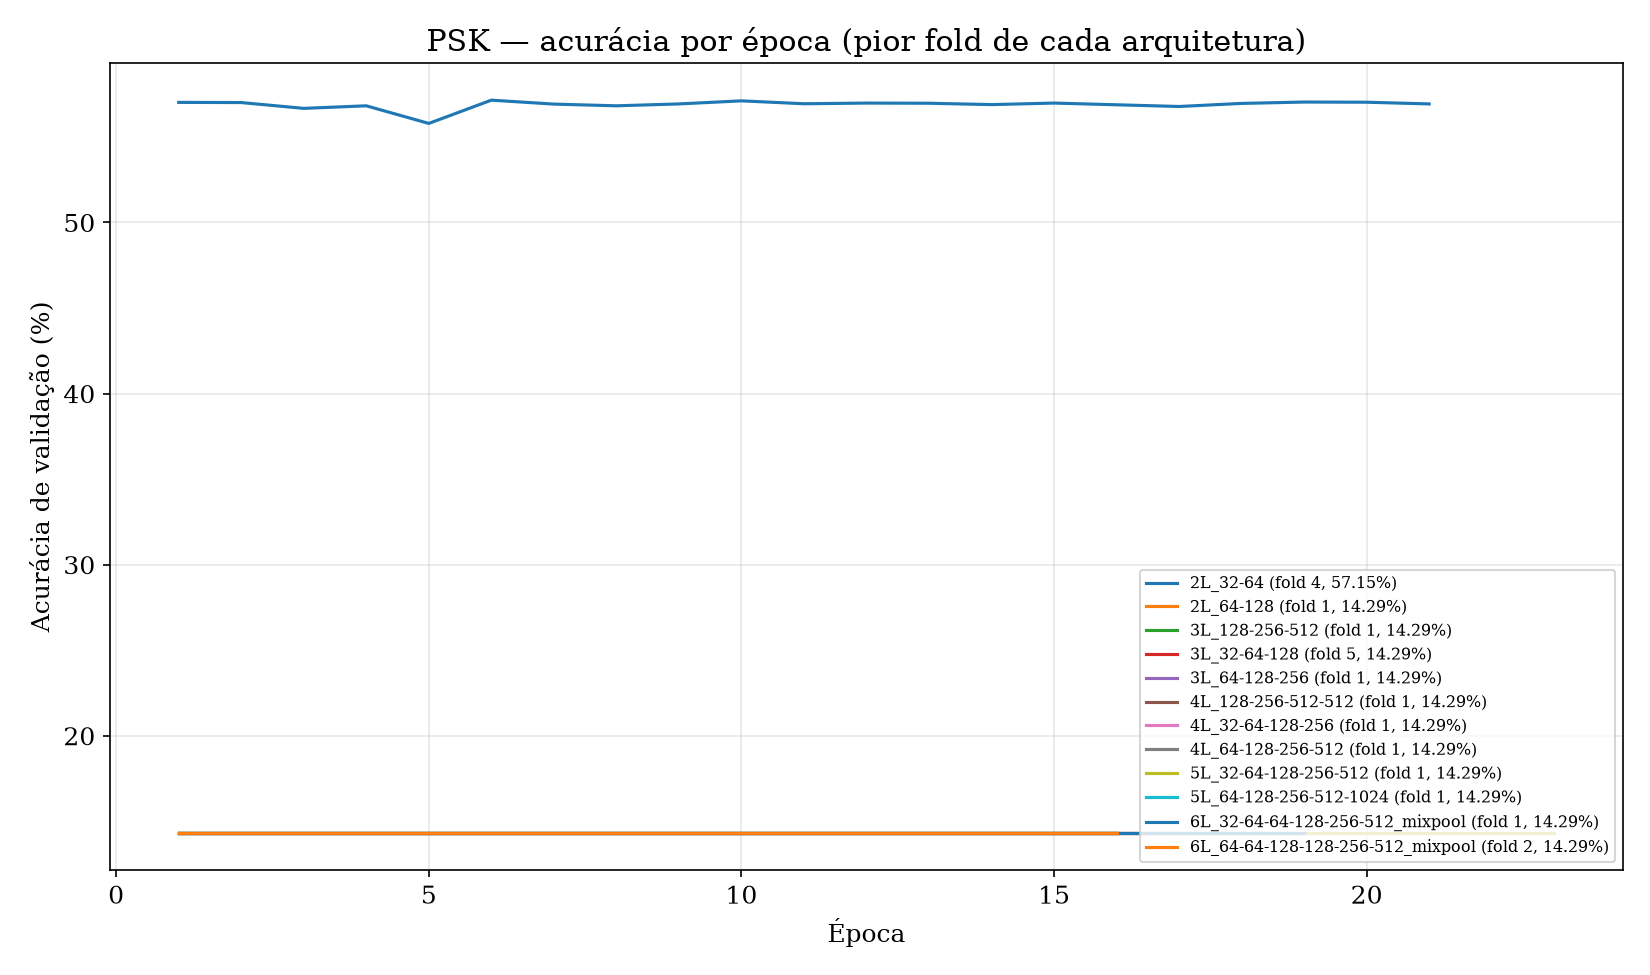
\includegraphics[width=0.96\textwidth,height=0.82\textheight,keepaspectratio]{report_figs/PSK_epochs_worst_fold_light.png}
\end{frame}
\begin{frame}{APSK --- acurácia por época (melhor fold de cada arquitetura)}
  \centering
  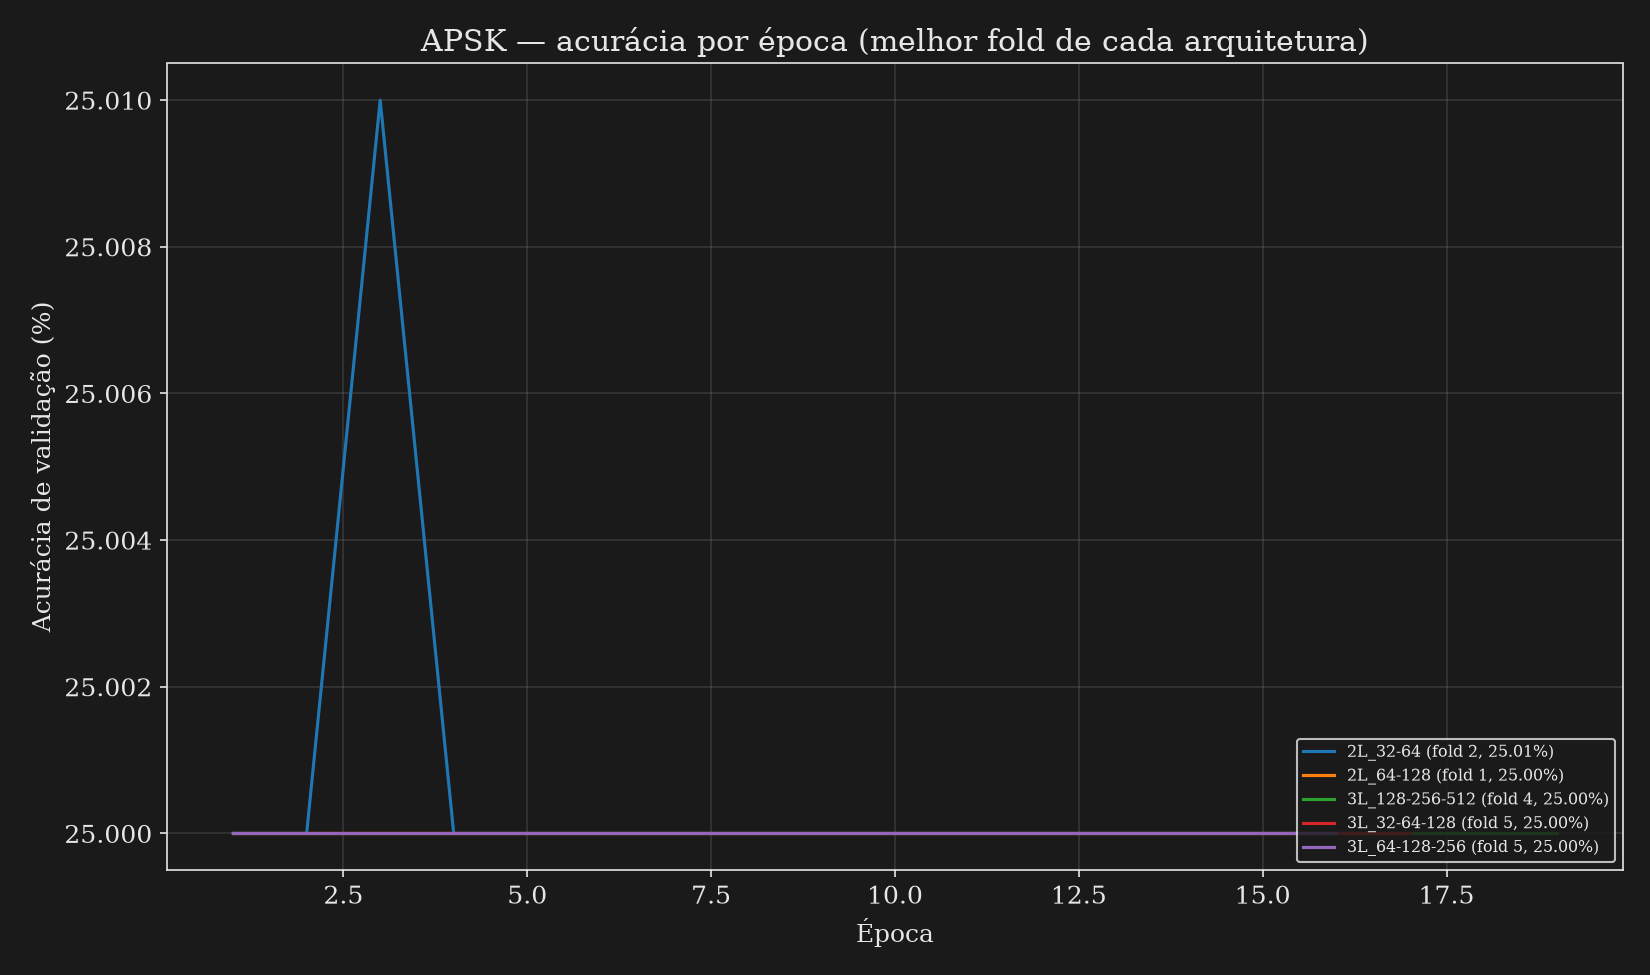
\includegraphics[width=0.96\textwidth,height=0.82\textheight,keepaspectratio]{kfold_analysis/APSK_epochs_best_fold.png}
\end{frame}
\begin{frame}{APSK --- acurácia por época (pior fold de cada arquitetura)}
  \centering
  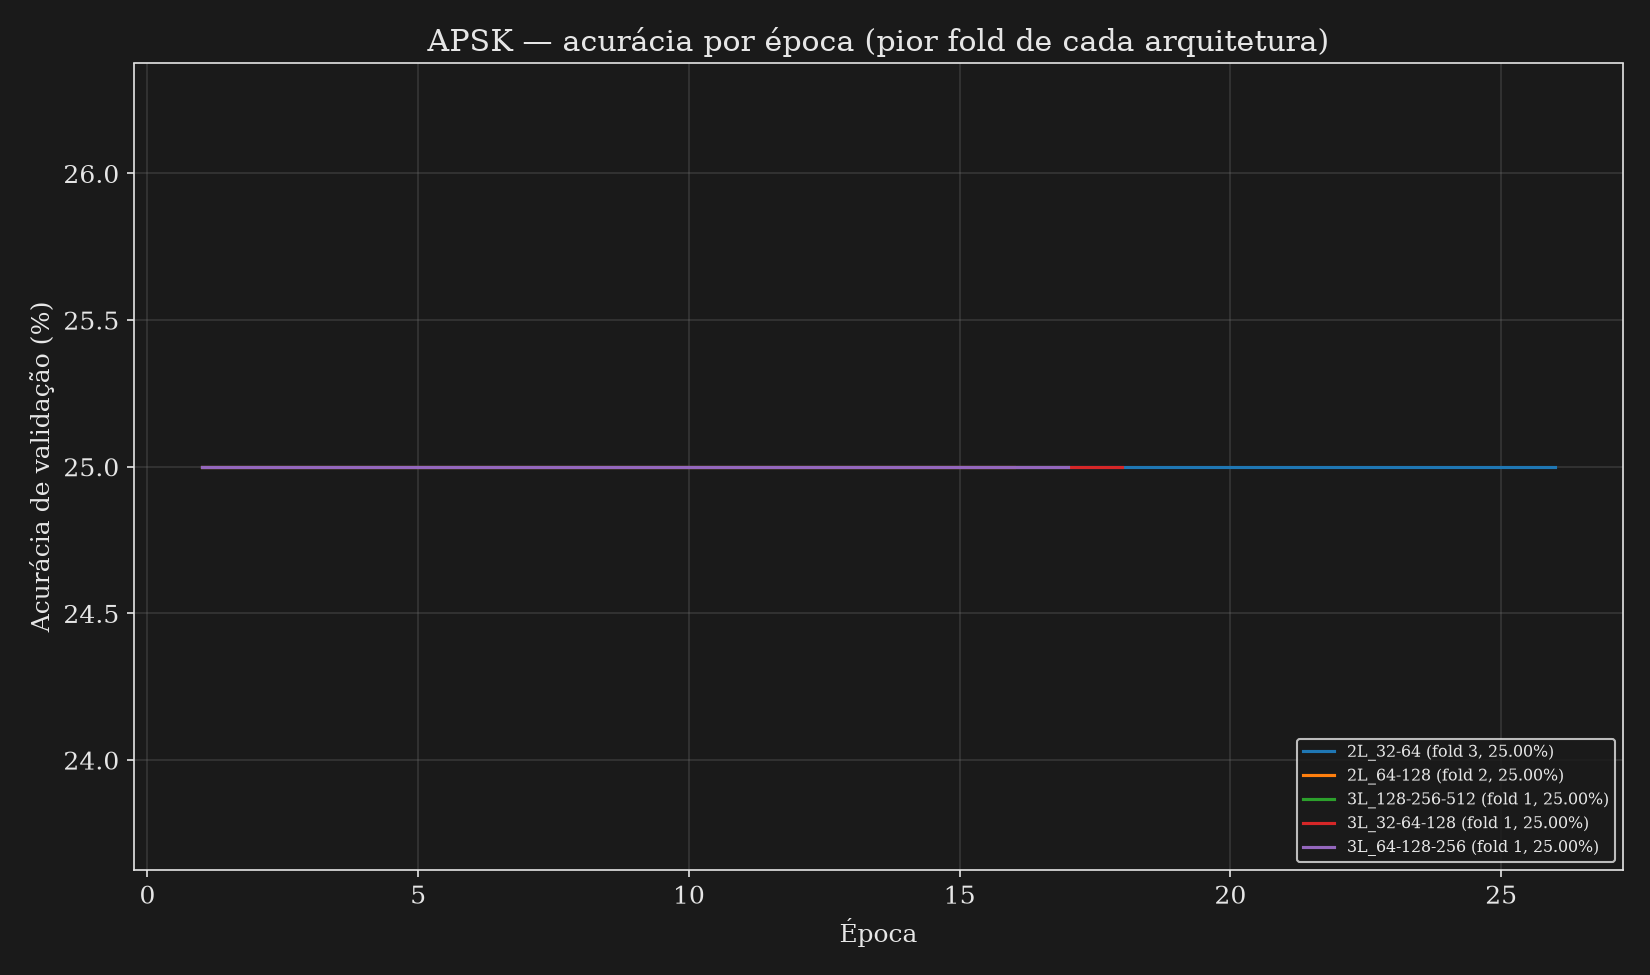
\includegraphics[width=0.96\textwidth,height=0.82\textheight,keepaspectratio]{kfold_analysis/APSK_epochs_worst_fold.png}
\end{frame}
\begin{frame}{APSK --- número de parâmetros $\times$ acurácia média}
  \centering
  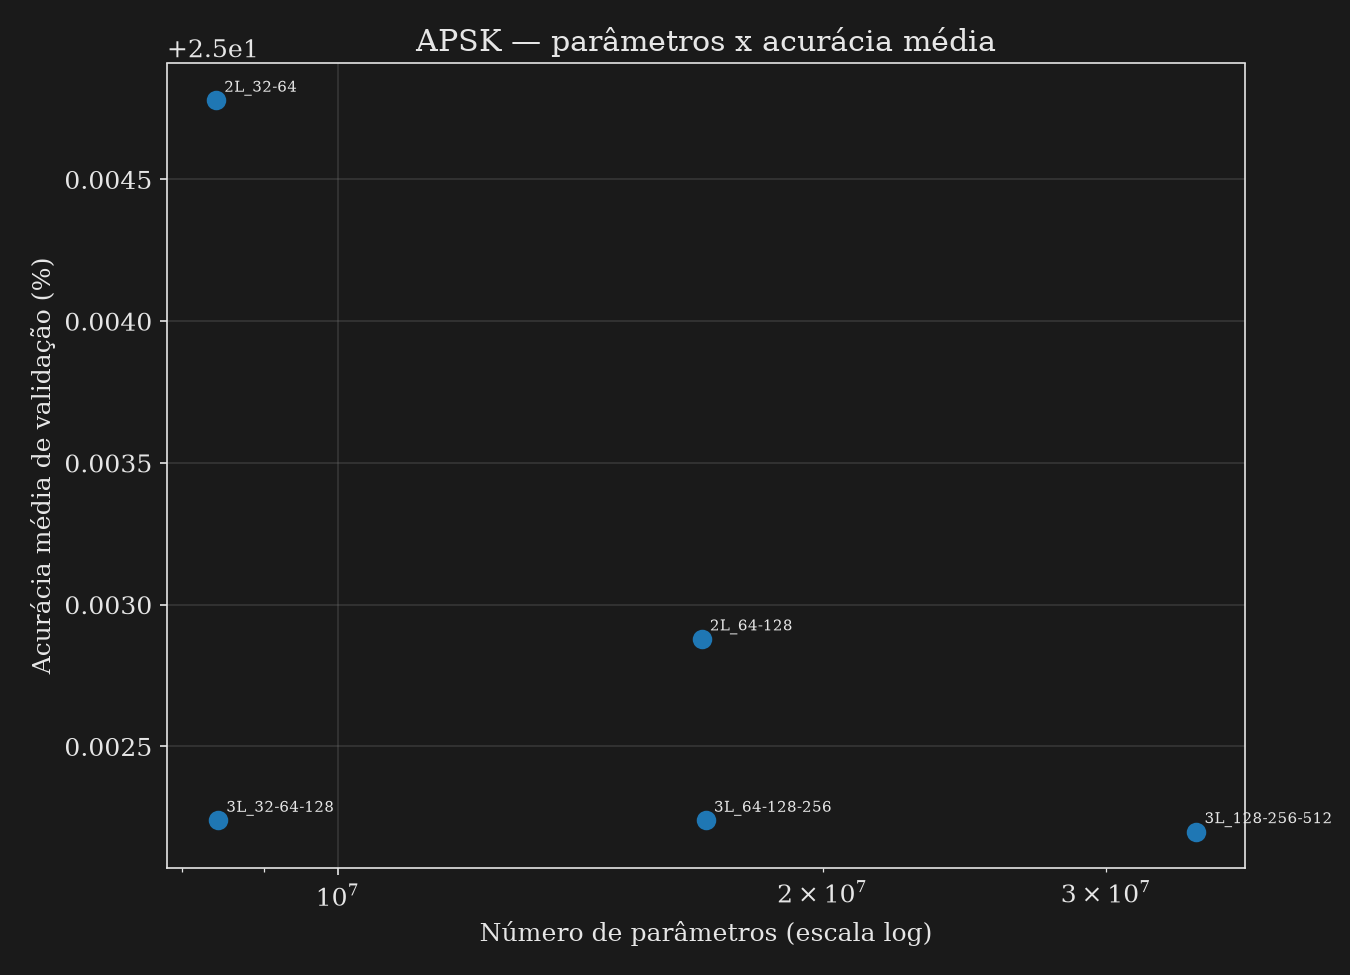
\includegraphics[width=0.96\textwidth,height=0.82\textheight,keepaspectratio]{kfold_analysis/APSK_params_vs_acc.png}
\end{frame}
\begin{frame}{QAM --- acurácia por época (melhor fold de cada arquitetura)}
  \centering
  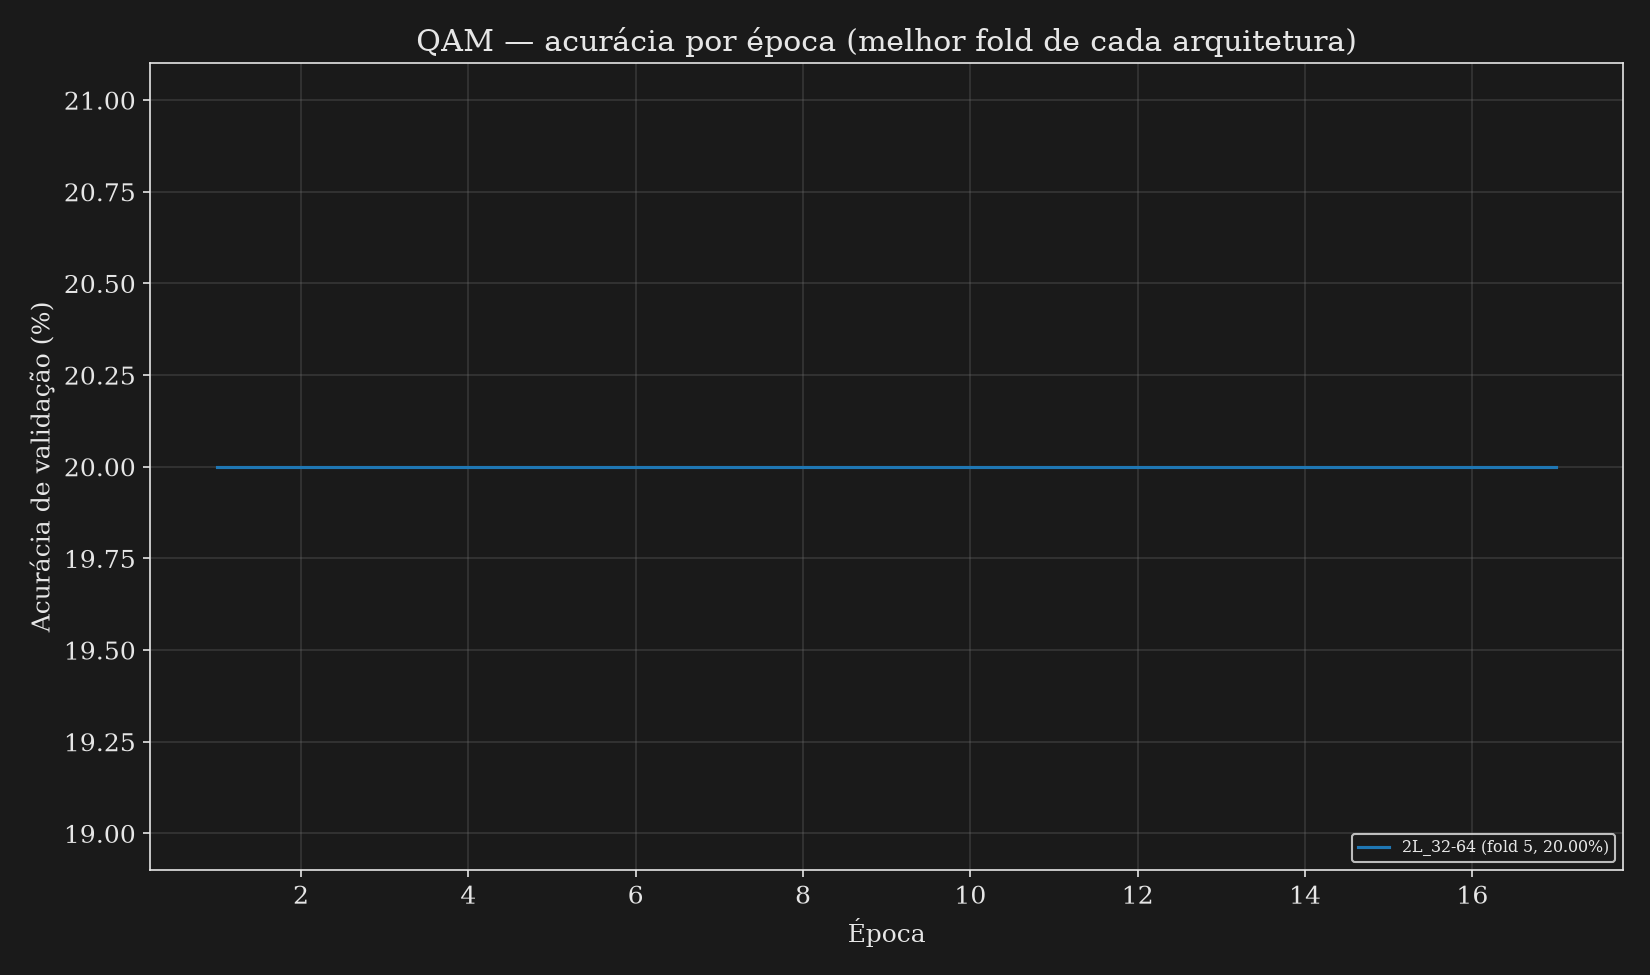
\includegraphics[width=0.96\textwidth,height=0.82\textheight,keepaspectratio]{kfold_analysis/QAM_epochs_best_fold.png}
\end{frame}
\begin{frame}{QAM --- acurácia por época (pior fold de cada arquitetura)}
  \centering
  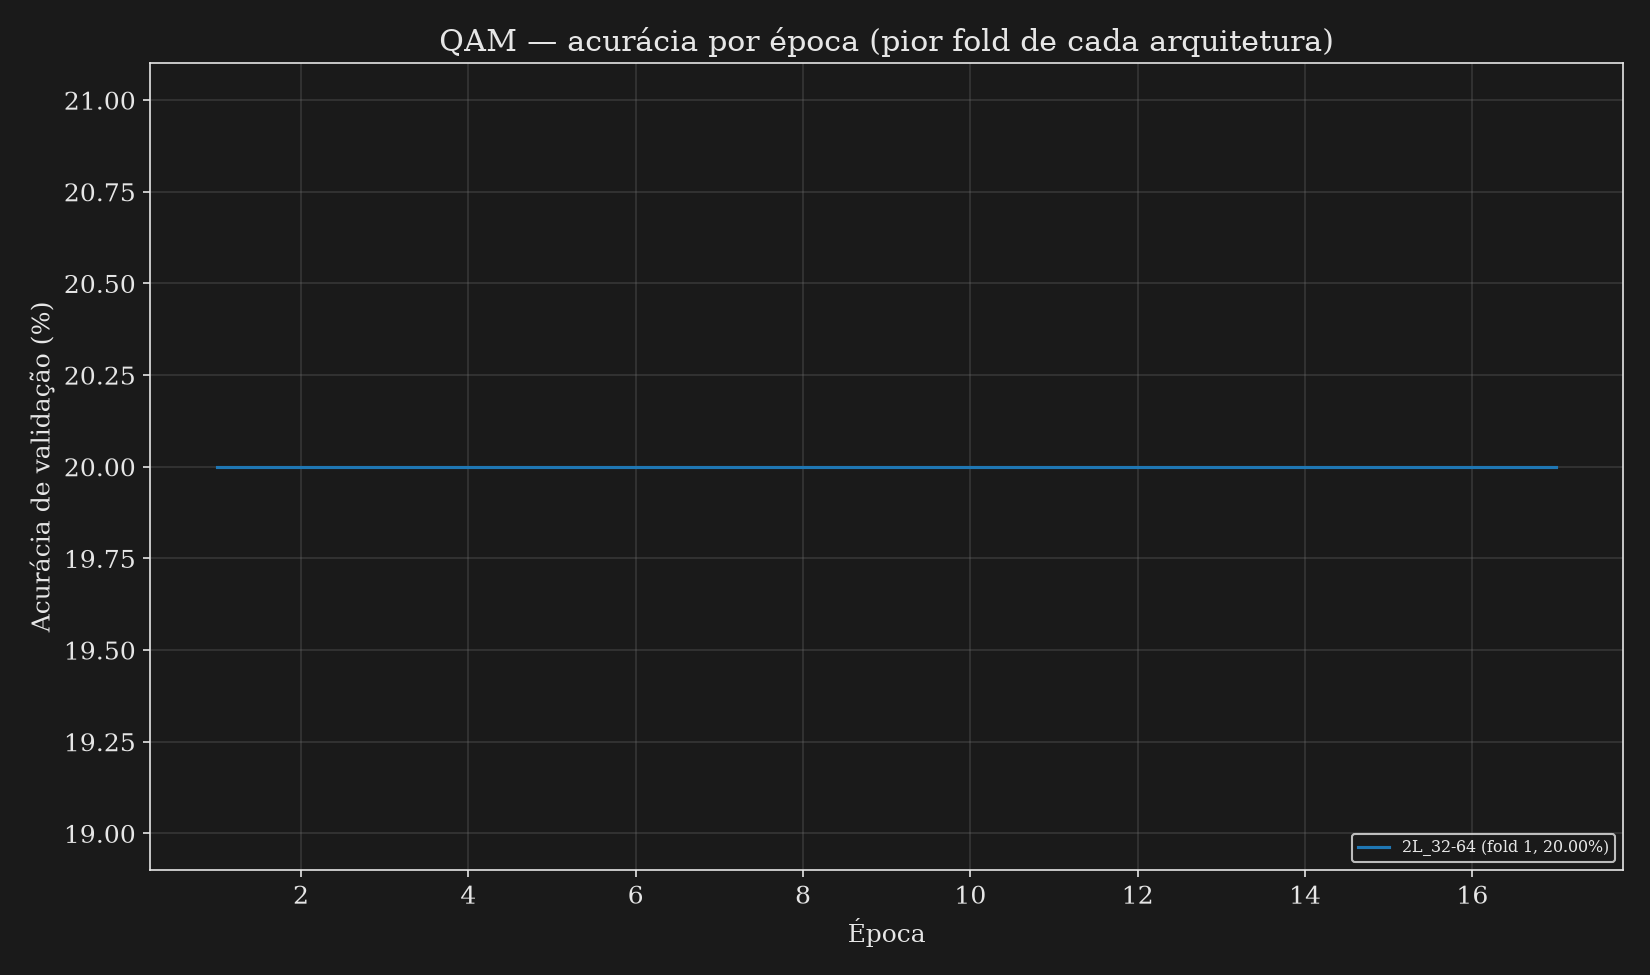
\includegraphics[width=0.96\textwidth,height=0.82\textheight,keepaspectratio]{kfold_analysis/QAM_epochs_worst_fold.png}
\end{frame}
\begin{frame}{QAM --- número de parâmetros $\times$ acurácia média}
  \centering
  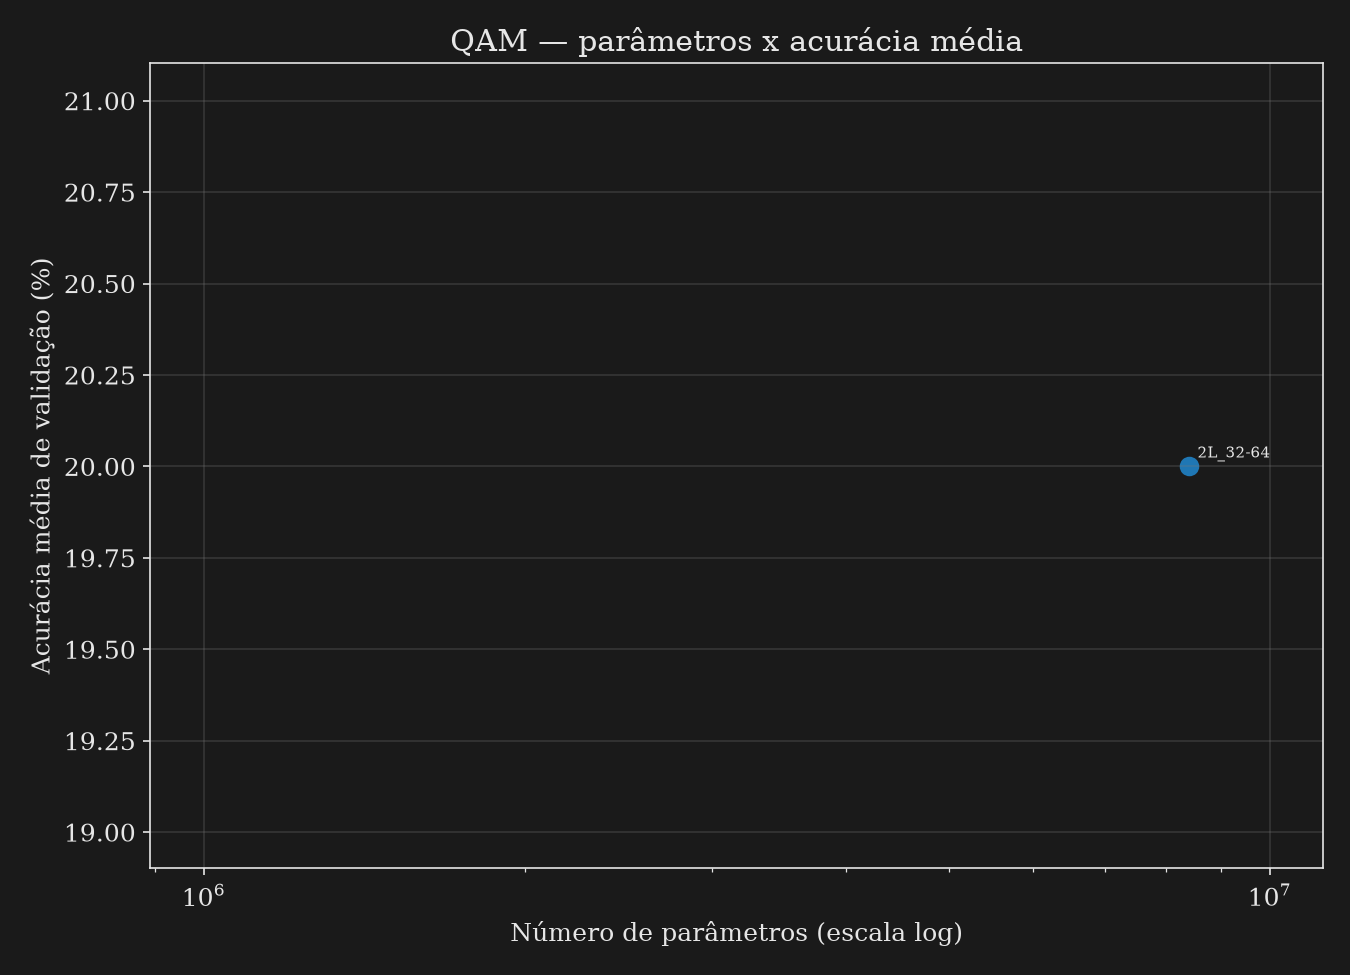
\includegraphics[width=0.96\textwidth,height=0.82\textheight,keepaspectratio]{kfold_analysis/QAM_params_vs_acc.png}
\end{frame}
\begin{frame}{AM --- acurácia por época (melhor fold de cada arquitetura)}
  \centering
  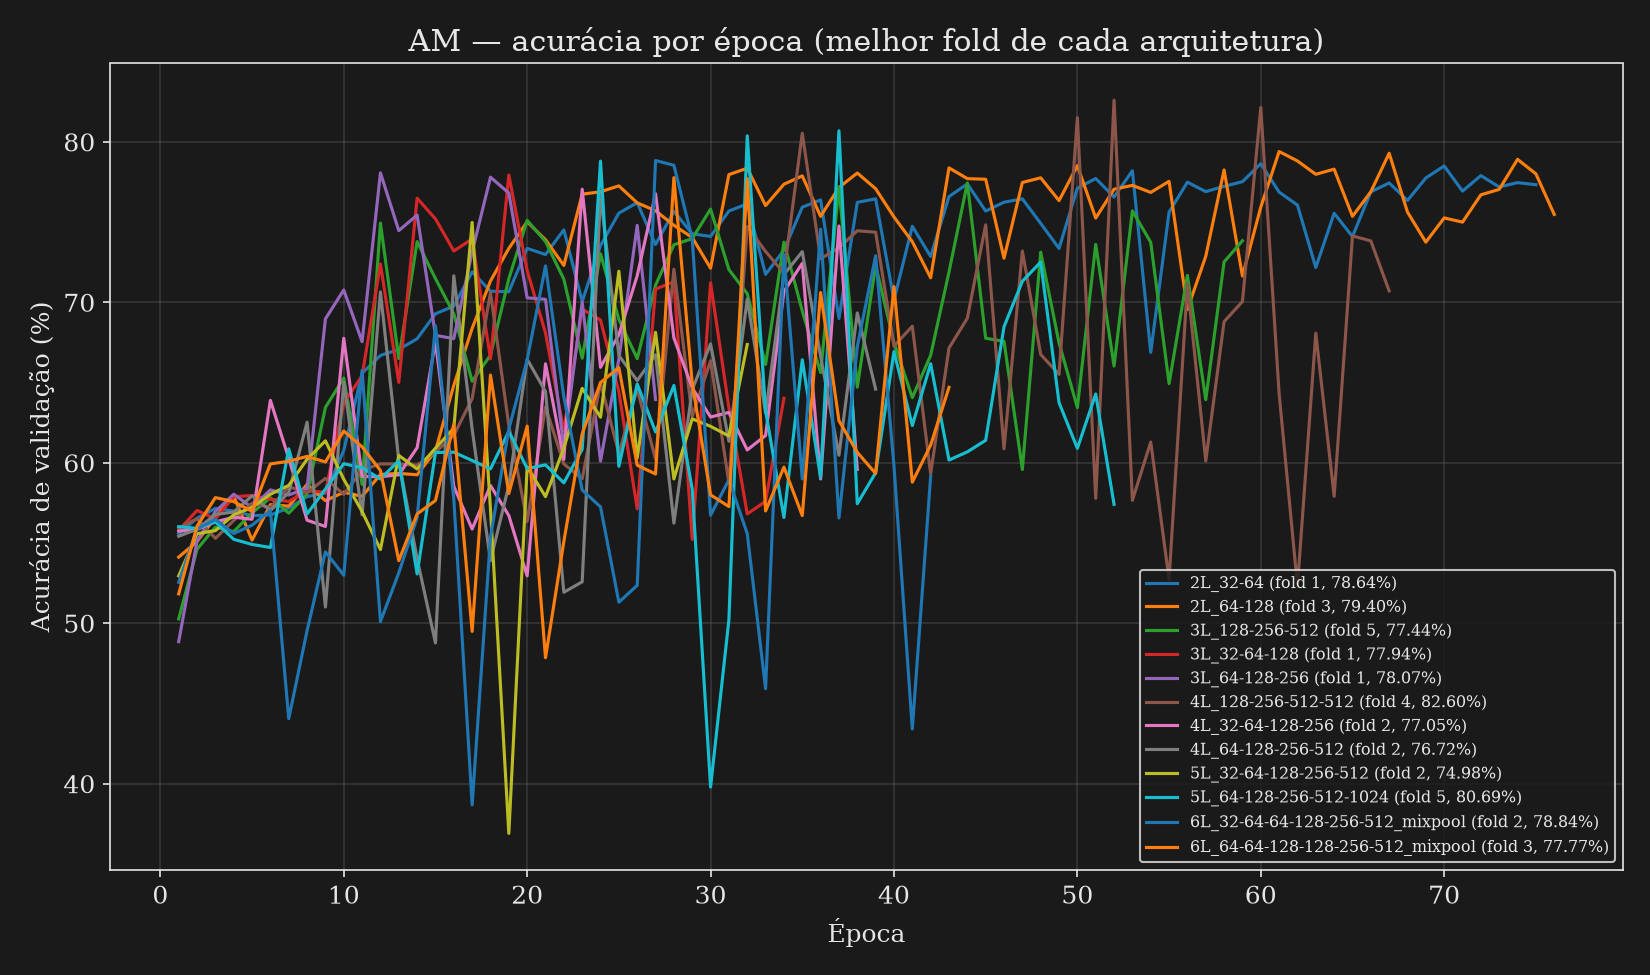
\includegraphics[width=0.96\textwidth,height=0.82\textheight,keepaspectratio]{kfold_analysis/AM_epochs_best_fold.png}
\end{frame}
\begin{frame}{AM --- acurácia por época (pior fold de cada arquitetura)}
  \centering
  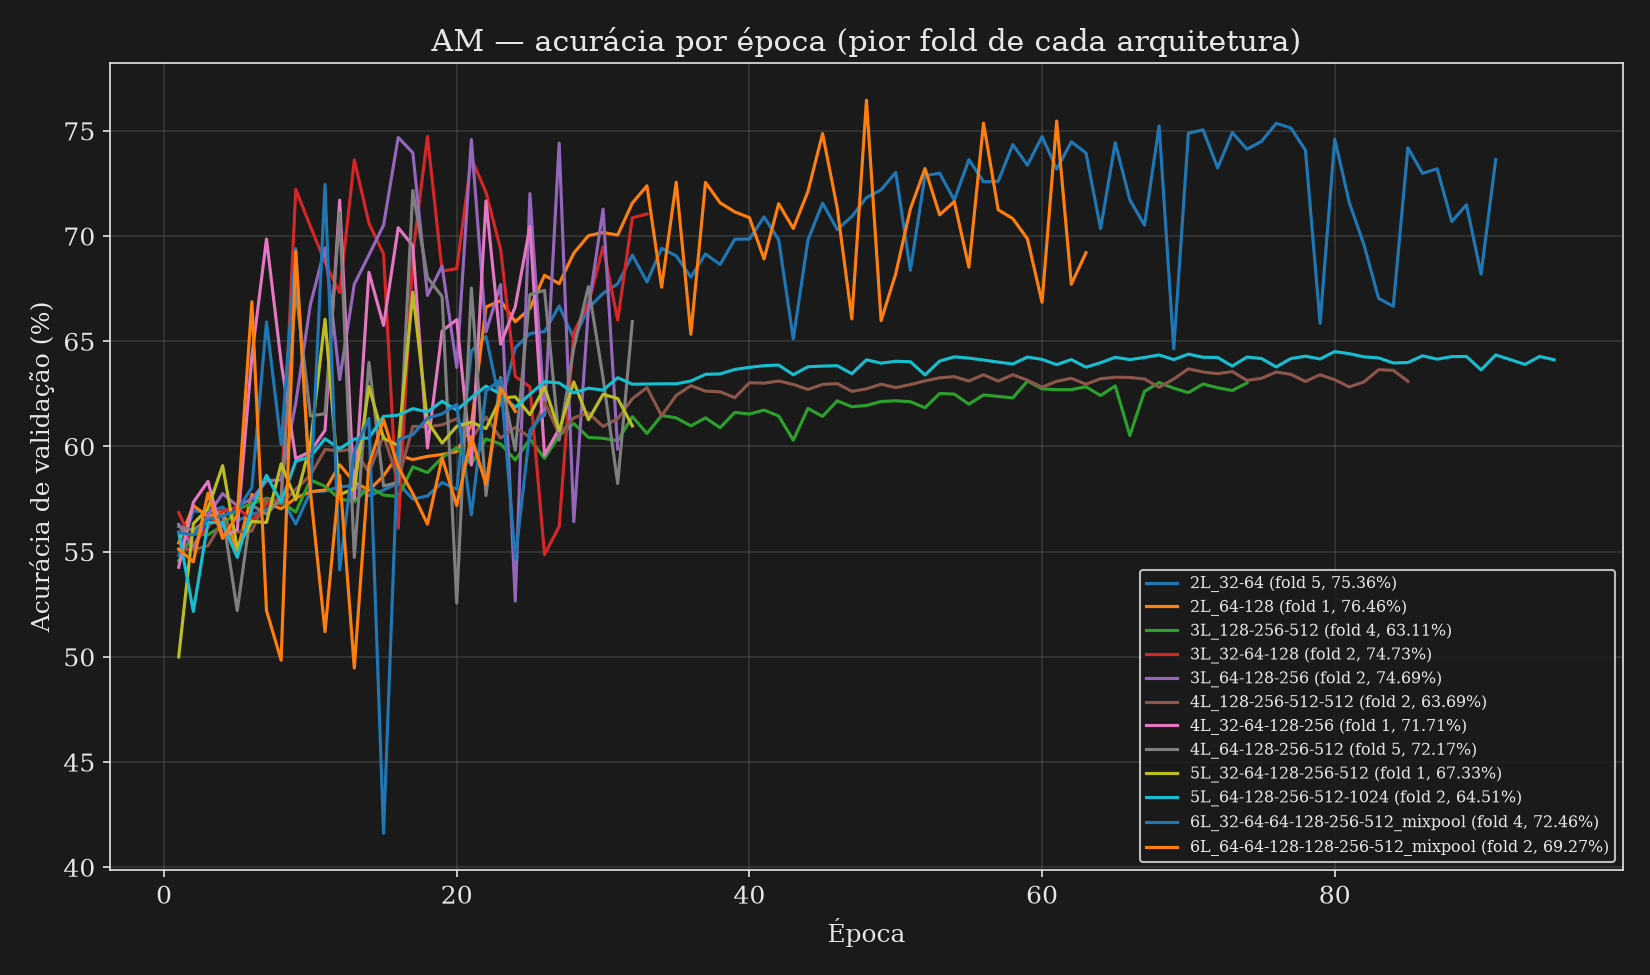
\includegraphics[width=0.96\textwidth,height=0.82\textheight,keepaspectratio]{kfold_analysis/AM_epochs_worst_fold.png}
\end{frame}
\begin{frame}{AM --- número de parâmetros $\times$ acurácia média}
  \centering
  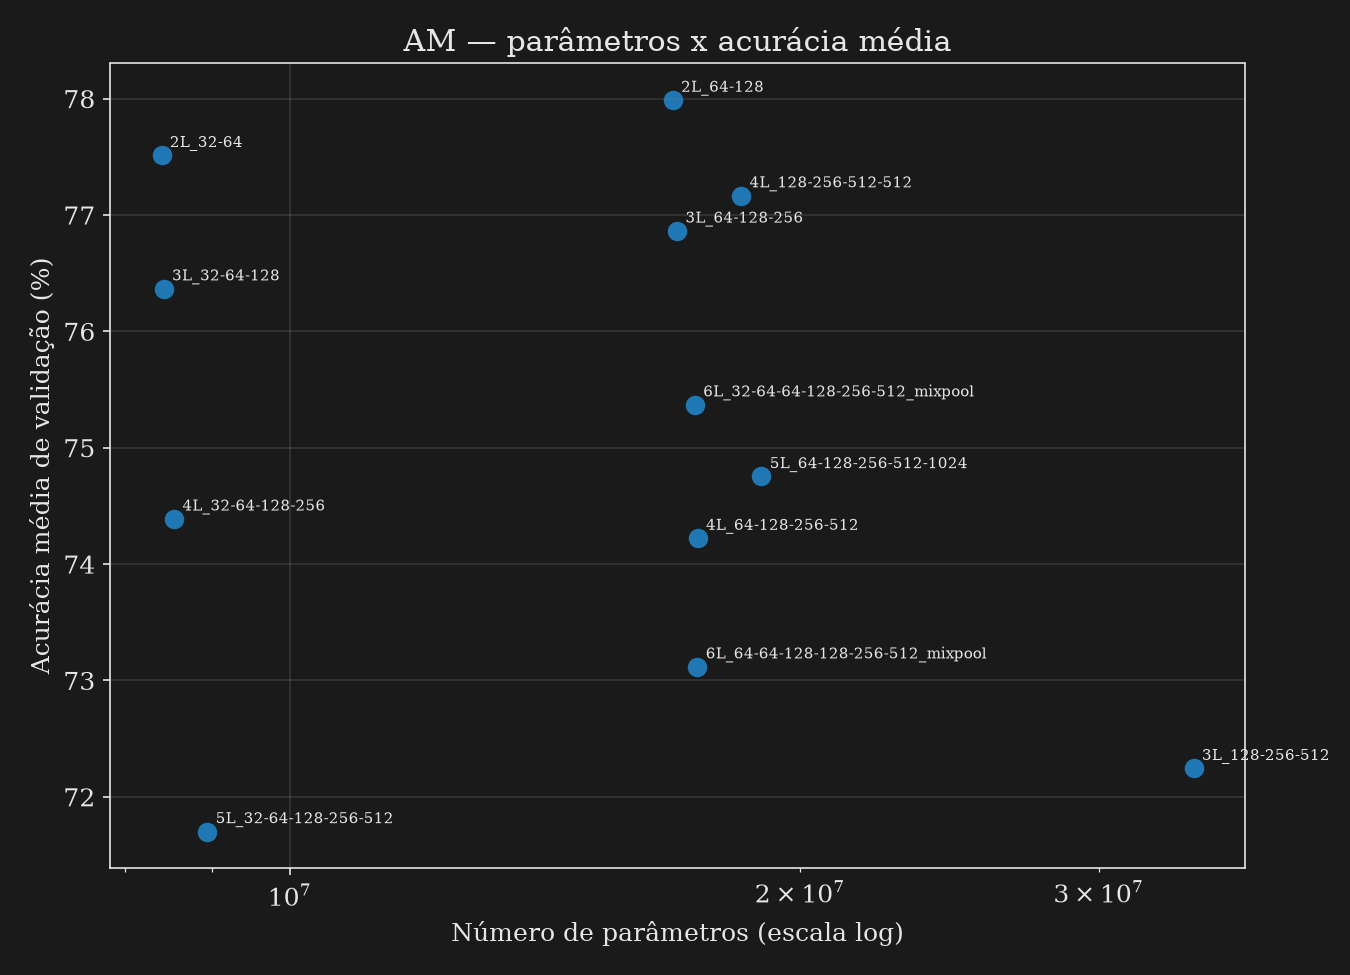
\includegraphics[width=0.96\textwidth,height=0.82\textheight,keepaspectratio]{kfold_analysis/AM_params_vs_acc.png}
\end{frame}

\begin{frame}{Resumo dos resultados por arquitetura (1/4)}
  \centering
  \small
  \begin{adjustbox}{max width=\textwidth}
  \begin{tabular}{llrrrrrr}
    \toprule
    Grupo & Arquitetura & Parâmetros & Folds & Média (\%) & Máx (\%) & Mín (\%) & Desv.\ (p.p.) \\
    \midrule
    AM & \texttt{2L\_64-128} & 16.822.212 & 5 & 77,99 & 79,40 & 76,46 & 0,95 \\
    AM & \texttt{2L\_32-64} & 8.402.148 & 5 & 77,51 & 78,64 & 75,36 & 1,14 \\
    AM & \texttt{4L\_128-256-512-512} & 18.457.988 & 5 & 77,17 & 82,60 & 63,69 & 6,99 \\
    AM & \texttt{3L\_64-128-256} & 16.921.284 & 5 & 76,86 & 78,07 & 74,69 & 1,20 \\
    AM & \texttt{3L\_32-64-128} & 8.427.108 & 5 & 76,37 & 77,94 & 74,73 & 1,04 \\
    AM & \texttt{6L\_32-64-64-128-256-512\_mixpool} & 17.334.564 & 5 & 75,37 & 78,84 & 72,46 & 2,22 \\
    AM & \texttt{5L\_64-128-256-512-1024} & 18.974.404 & 5 & 74,75 & 80,69 & 64,51 & 5,80 \\
    AM & \texttt{4L\_32-64-128-256} & 8.546.916 & 5 & 74,39 & 77,05 & 71,71 & 2,05 \\
    AM & \texttt{4L\_64-128-256-512} & 17.398.468 & 5 & 74,22 & 76,72 & 72,17 & 1,63 \\
    AM & \texttt{6L\_64-64-128-128-256-512\_mixpool} & 17.394.948 & 5 & 73,12 & 77,77 & 69,27 & 3,27 \\
    AM & \texttt{3L\_128-256-512} & 34.118.532 & 5 & 72,24 & 77,44 & 63,11 & 6,02 \\
    AM & \texttt{5L\_32-64-128-256-512} & 8.941.668 & 5 & 71,70 & 74,98 & 67,33 & 2,72 \\
    \bottomrule
  \end{tabular}
  \end{adjustbox}
\end{frame}

\begin{frame}{Resumo dos resultados por arquitetura (2/4)}
  \centering
  \small
  \begin{adjustbox}{max width=\textwidth}
  \begin{tabular}{llrrrrrr}
    \toprule
    Grupo & Arquitetura & Parâmetros & Folds & Média (\%) & Máx (\%) & Mín (\%) & Desv.\ (p.p.) \\
    \midrule
    APSK & \texttt{2L\_32-64} & 8.402.148 & 5 & 25,00 & 25,01 & 25,00 & 0,00 \\
    APSK & \texttt{2L\_64-128} & 16.822.212 & 5 & 25,00 & 25,00 & 25,00 & 0,00 \\
    APSK & \texttt{3L\_32-64-128} & 8.427.108 & 5 & 25,00 & 25,00 & 25,00 & 0,00 \\
    APSK & \texttt{3L\_64-128-256} & 16.921.284 & 5 & 25,00 & 25,00 & 25,00 & 0,00 \\
    APSK & \texttt{3L\_128-256-512} & 34.118.532 & 4 & 25,00 & 25,00 & 25,00 & 0,00 \\
    ASK* & \texttt{6L\_64-64-128-128-256-512\_mixpool} & 17.394.435 & 5 & 97,80 & 97,93 & 97,73 & 0,07 \\
    ASK* & \texttt{6L\_32-64-64-128-256-512\_mixpool} & 17.334.051 & 5 & 97,71 & 97,76 & 97,64 & 0,04 \\
    ASK* & \texttt{5L\_32-64-128-256-512} & 8.941.155 & 5 & 97,70 & 97,81 & 97,57 & 0,08 \\
    ASK* & \texttt{5L\_64-128-256-512-1024} & 18.973.891 & 5 & 97,66 & 97,82 & 97,45 & 0,15 \\
    ASK* & \texttt{4L\_32-64-128-256} & 8.546.403 & 5 & 97,62 & 97,73 & 97,57 & 0,07 \\
    ASK* & \texttt{4L\_64-128-256-512} & 17.397.955 & 5 & 97,62 & 97,69 & 97,56 & 0,05 \\
    ASK* & \texttt{4L\_128-256-512-512} & 18.457.475 & 5 & 97,62 & 97,69 & 97,58 & 0,04 \\
    \bottomrule
  \end{tabular}
  \end{adjustbox}
  \par\vspace{2mm}{\scriptsize * dados do relatório (backups locais); não disponíveis no Drive.}
\end{frame}

\begin{frame}{Resumo dos resultados por arquitetura (3/4)}
  \centering
  \small
  \begin{adjustbox}{max width=\textwidth}
  \begin{tabular}{llrrrrrr}
    \toprule
    Grupo & Arquitetura & Parâmetros & Folds & Média (\%) & Máx (\%) & Mín (\%) & Desv.\ (p.p.) \\
    \midrule
    ASK* & \texttt{3L\_64-128-256} & 16.920.771 & 5 & 97,09 & 97,22 & 96,96 & 0,10 \\
    ASK* & \texttt{3L\_128-256-512} & 34.118.019 & 5 & 97,07 & 97,35 & 96,90 & 0,16 \\
    ASK* & \texttt{3L\_32-64-128} & 8.426.595 & 5 & 96,95 & 97,19 & 96,81 & 0,14 \\
    ASK* & \texttt{2L\_64-128} & 16.821.699 & 5 & 93,74 & 94,30 & 93,03 & 0,42 \\
    ASK* & \texttt{2L\_32-64} & 8.401.635 & 5 & 93,28 & 93,95 & 92,99 & 0,36 \\
    PSK* & \texttt{2L\_32-64} & 8.403.687 & 5 & 68,21 & 83,51 & 57,15 & 9,61 \\
    PSK* & \texttt{3L\_32-64-128} & 8.428.647 & 5 & 53,26 & 84,92 & 14,29 & 26,55 \\
    PSK* & \texttt{4L\_32-64-128-256} & 8.548.455 & 5 & 46,89 & 96,00 & 14,29 & 39,94 \\
    PSK* & \texttt{6L\_32-64-64-128-256-512\_mixpool} & 17.336.103 & 5 & 42,10 & 96,22 & 14,29 & 34,95 \\
    PSK* & \texttt{2L\_64-128} & 16.823.751 & 5 & 36,91 & 42,90 & 14,29 & 11,31 \\
    PSK* & \texttt{5L\_32-64-128-256-512} & 8.943.207 & 5 & 30,61 & 95,91 & 14,29 & 32,65 \\
    PSK* & \texttt{6L\_64-64-128-128-256-512\_mixpool} & 17.396.487 & 5 & 25,71 & 71,39 & 14,29 & 22,84 \\
    \bottomrule
  \end{tabular}
  \end{adjustbox}
  \par\vspace{2mm}{\scriptsize * dados do relatório (backups locais); não disponíveis no Drive.}
\end{frame}

\begin{frame}{Resumo dos resultados por arquitetura (4/4)}
  \centering
  \small
  \begin{adjustbox}{max width=\textwidth}
  \begin{tabular}{llrrrrrr}
    \toprule
    Grupo & Arquitetura & Parâmetros & Folds & Média (\%) & Máx (\%) & Mín (\%) & Desv.\ (p.p.) \\
    \midrule
    PSK* & \texttt{3L\_128-256-512} & 34.120.071 & 5 & 20,00 & 42,85 & 14,29 & 11,42 \\
    PSK* & \texttt{3L\_64-128-256} & 16.922.823 & 5 & 14,29 & 14,29 & 14,29 & 0,00 \\
    PSK* & \texttt{4L\_64-128-256-512} & 17.400.007 & 5 & 14,29 & 14,29 & 14,29 & 0,00 \\
    PSK* & \texttt{4L\_128-256-512-512} & 18.459.527 & 5 & 14,29 & 14,29 & 14,29 & 0,00 \\
    PSK* & \texttt{5L\_64-128-256-512-1024} & 18.975.943 & 5 & 14,29 & 14,29 & 14,29 & 0,00 \\
    QAM & \texttt{2L\_32-64} & 8.402.661 & 5 & 20,00 & 20,00 & 20,00 & 0,00 \\
    \bottomrule
  \end{tabular}
  \end{adjustbox}
  \par\vspace{2mm}{\scriptsize * dados do relatório (backups locais); não disponíveis no Drive.}
\end{frame}

\end{document}
